\documentclass{article}

\usepackage{graphicx} % Required for inserting images
\usepackage{amssymb}
\usepackage{lipsum}
\usepackage[affil-it]{authblk}
\usepackage{multicol}
\setlength{\columnsep}{1cm}
\usepackage{lipsum}% for dummy text
\usepackage[utf8]{inputenc}
\usepackage{fullpage}
\usepackage{titlesec}
\usepackage{hyperref}
\usepackage{xcolor}
\usepackage{amsmath}
\usepackage{varioref}
\usepackage{booktabs}
\usepackage{verbatim}
\usepackage{float}
\usepackage{placeins}
\usepackage{caption}
\usepackage{subcaption}
\usepackage{url}



\hypersetup{
    colorlinks=true,
    linkcolor=blue,  
    citecolor=blue,  
    urlcolor=blue   
}


\titleformat{\subsection}{\normalfont\fontsize{10}{12}\itshape\bfseries}{\thesubsection}{1em}{}
\titleformat{\subsubsection}{\normalfont\fontsize{9}{11}\itshape\bfseries}{\thesubsubsection}{1em}{}



\title{\textbf{Predicting learning disorder rate in children with ASD traits}}
\author{\textbf{Fahrin Hossain Sunaira, Shanila Nehlin, S.A.M. Zahin Abdal, Shakirul Islam Leon}}
\affil{Department of Electrical and Computer Engineering, North South University, Dhaka, 1229, Bangladesh}
\date{}


\begin{document}


\maketitle

\hrule
\begin{abstract}
\noindent Learning disorder is common among children with ASD. Although autism itself is not a learning disability, it can significantly affect a child’s ability to process and retain information. And as a result, hinders their academic and social progress. Early diagnosis of children who may have chances of developing learning disorder often helps to provide effective treatment. This research aims to develop mechanisms to detect and predict the learning disorder in children with ASD traits aged from 1 to 18 years old. In this work, the dataset has been obtained from Kaggle, which consisted primarily of 1985 different set of values. After data preprocessing, we obtained our final dataset with 1937 values. In total, nine machine learning algorithms were employed to predict whether a child with ASD traits has probability of developing learning disorder or not. Two hyperparameter optimizers were employed to improve the predictability. Accuracies of 99.48\% were obtained by both decision tree and random tree classifier. Finally, LIME, an explainable AI framework, was applied to interpret and retrace the prediction output of the machine learning models.
\vspace{\baselineskip}
\end{abstract}
\hrule
\vspace{3\baselineskip}
\setlength{\parindent}{24pt}




\begin{multicols}{2}

\section{Introduction}
\hspace*{\parindent}  Autism spectrum disorder (ASD) is a neurodevelopmental disorder characterized by persistent difficulties in social communication and interaction and restrictive, repetitive, and stereotyped patterns of behavior, activities, and interests \cite{rosello2018adhd}. It is referred to as a neurological and developmental disorder that affects how people interact with others, communicate, learn, and behave \cite{yamamoto2021children}.\\
\hspace*{\parindent} Individuals with ASD experience difficulties in three domains: reciprocal social interaction, stereotyped and repetitive behaviors and verbal and nonverbal communication due to learning disorder \cite{starr2006schools}. Out of these 3 major difficulties, our study aims to focus on the learning disorder faced by the children. It has been reported that around 4 in 10 autistic people have a learning disorder \cite{autistica2023learningdisability}. A learning disorder affects the children in different ways. Common difficulties include: 
\begin{itemize}
    \item adapting behaviour to different situations
    \item interacting with others
    \item controlling behaviour
\end{itemize} 
\hspace*{\parindent} Children with ASD may develop language at a later age than others, use language differently compared to their peers, or may not communicate with language at all. ASD also affects joint attention, the use of social cues, gestures, and eye contact to communicate with others, which has profound impacts on both learning and socialization \cite{SpectrumofHope2023AutismLearningDisorders}. Learning disorders “alter brain functioning in a manner which affects cognitive processes” related to learning. A condition like dyslexia, for instance, affects an individual’s ability to read via challenges with word recognition and decoding. Common learning disorders include dyslexia, which affects reading; dyscalculia, which affects mathematics; and dysgraphia, which affects writing \cite{sun2019learning}. 
\hspace*{\parindent} The findings of these studies on children with ASD are concerning and require appropriate action. As a step toward that, this study attempts to take the first step towards understanding the learning disorder rate in children with ASD traits where machine learning techniques have been utilized to tackle this issue, and prevent the issue from worsening further in the near future. Firstly, we obtained our dataset from Kaggle, where the data consists of different quantities and factors which are characteristics of ASD in children. The data in the dataset is collected from AUTISM RESEARCH: UNIVERSITY OF ARKANSAS Computer Science Department to analyze the disease conditions and predict them beforehand. Major contributions of our work are illustrated below: 
\begin{itemize}
    \item A new scale has been created to measure the occurrence of learning disorder in children with ASD traits as either yes or no.
    \item Machine learning algorithms have been applied to predict learning disorder rates. 
    \item Hyperparameter optimizers and feature selection methods are used to improve the performance of these models. 
    \item LIME, an explainable AI tool, has been used to understand the final predictions provided by machine learning models. 
    \item The created models were also cross-validated, demonstrating the robustness of the models.
\end{itemize}
\hspace*{\parindent} The following is the order in which this article is organized. Literature review, that is, related works are addressed in Section \textbf{2}. Section \textbf{3} focuses discussion of the methodology adopted in this work. Section \textbf{4} examines the acquired outcomes, that is, the result analysis. Section \textbf{5} focuses on the discussion of our study. Section \textbf{6} discusses the limitation of this work and finally, Section \textbf{7} includes a conclusion with remarks on our future work.

\section{Literature Review}
\hspace*{\parindent}According to the International Classification of Functioning (ICF) by the World Health Organization, ``functioning'' encompasses all aspects of an individual’s life, going beyond just ``adaptive functioning'' or ``cognitive functioning''. Accurately measuring Neurodevelopmental Disorders(NDD) such as Specific Learning Disorder, Attention-Deficit/Hyperactivity Disorder(ADHD), and Autism is crucial for creating a tool that can enhance the daily lives of affected individuals. Learning disabilities impact the brain's capacity to receive, process, interpret, or retain information, leading to challenges in a child's ability to learn at a pace similar to that of individuals without such learning difficulties \cite{sood2013construction}. Some experts have found a correlation between learning disabilities and brain development before and after birth \cite{cruickshank1975perceptual}. Consequently, factors like low birth weight, oxygen deprivation, or premature birth may be contributing factors to the occurrence of learning disabilities. Additionally, young children who experience head injuries may be susceptible to developing these conditions. Infants and toddlers are also vulnerable to the effects of environmental toxins or harmful substances. A study reported that learning disabilities can be divided into verbal and nonverbal. Individuals with verbal learning disabilities, also known as dyslexia, face difficulty with recognizing or processing letters, which may be extended to spoken words or sounds associated with them \cite{lerner1997learning}. Whereas, children with non-verbal learning disabilities may find it challenging to make sense of what they see. Examinations of postmortem dyslexic brains have revealed alterations in brain structure, including ectopias, microgyri, and asymmetry \cite{caylak2009neurobiological}.\\\\
\hspace*{\parindent}Researchers are continuously studying to find the most suitable tools for identifying  Learning Disorders(LD) among individuals. A study conducted by Australian clinicians to select the characteristics of such a tool concluded that they consider various factors, including ease of use, feasibility, fairness, holism, and usefulness, when choosing an assessment of a functioning tool for children with neurodevelopmental conditions (NDC) \cite{d2022australian}. A research investigation that integrated the Frequency Following Response(FFR) was employed to develop a diagnostic instrument for the detection of Learning Disorders (LDs) in individuals. The findings demonstrated that individuals with learning disorders exhibited neural discrimination that was both unstable and characterized by greater variability. These individuals displayed diminished subcortical performance in processing spectral components, a less precise depiction of the extent and type of neural coding, a prolonged transition period, and notably longer response latencies compared to their counterparts without learning disorders \cite{cordeiro2020assessment}. The Learning Disabilities Checklist has been used in numerous studies to differentiate children with and without disabilities. This checklist consists of 91 items measuring six domains of LDs: Gross and Fine Motor Skills (8 items), Language (17 items), Reading (15 items), Writing (12 items), Mathematics (12 items), Social Emotional Functioning (10 items), Attention (8 items), and others (10 items). Selected 39 items measured Reading (15 items), Writing (12 items), and Mathematical Disabilities (12 items). This method of screening for LD  has been previously followed by researchers across Pakistan and other countries \cite{malik2013screening}. One such study demonstrated 39 items from the checklist showed that the response to the statements significantly differentiated children with and without disabilities \cite{ashraf2014validation}. The findings are consistent with the observations of Rutter et al.\cite{rutter2004gender}, who found that boys have more prevalence of LDs as compared to girls. It is evident that there is a pressing need for a faster and more efficient method for the detection of Learning Disorders(LD). This study, therefore, endeavors to develop and assess a machine-learning tool intended for use by teachers, parents, and other individuals, with the aim of swiftly and accurately identifying learning disorders among individuals.




\section{Methodology}
\hspace*{\parindent}Fig. \ref{mapping} shows the primary steps taken in this research. Following the acquirement of the dataset, the dataset is preprocessed so that it is in a format conducive to machine learning algorithms to operate on, after splitting the data into training and test sets. Other methods will also be applied as seen in the figure, to get a conclusive result for the learning rate in the children with ASD traits.

\subsection{Problem Formulation}
\hspace*{\parindent}One of the foremost step into our study was to decide what to predict with our dataset. There were several factors which are normally seen in children with ASD traits, and the dataset obtained had many notable features like depression, social responsiveness scale, global developmental delay which are characteristics of children with ASD traits, but out of those features learning disorder seemed to be a very important factor, since it might affect these children a lot in the near future, and they might learn not to communicate at all. Thereby, we decided to make learning disorder the target and predict the learning disorder rate in children with ASD traits, so the ones who have a higher probability will be provided with appropriate clinical actions.

\subsection{Data Acquisition}
\hspace*{\parindent}Our dataset was acquired from Kaggle(\url{https://www.kaggle.com/datasets/uppulurimadhuri/dataset}), and this particular dataset was collected initially by AUTISM RESEARCH: UNIVERSITY OF ARKANSAS Computer Science Department for their research. This dataset contains 1985 rows and 28 columns, and the age range of the children is between 1 to 18 years, and they are mostly from Europe, Asia and Middle East. There are many features that are checked within candidates, and the notable columns incldude features such as -- 
``Social\_Responsiveness\_Scale'', ``Speech Delay/Language Disorder'', ``Learning disorder'', ``Genetic\_Disorders'', ``Depression'', ``Global developmental delay/Intellectual disability'', ``Social/Behavioural Issues'', ``Childhood Autism Rating Scale'', ``Anxiety\_disorder'', ``Jaundice'', ``Family\_mem\_with\_ASD''. These features will thereby be modified and used for the outcome of our prediction.

\subsection{Data Preprocessing}
\hspace*{\parindent}The data cleaning, organizing, visualizing have been described exhaustively in this section.

\subsubsection{Data Cleaning}
\hspace*{\parindent}The dataset we obtained contained primarily of 1985 rows and 28 columns. Amongst that we found out that there were null values present in the ‘Qchat\_10\_score’ and ‘Social/Behavioural Issues’ columns. So, we subsequently dropped the rows have the rows having null values for this, which therefore resulted in the dataset now consisting of 1937 rows and 28 columns.

\end{multicols}
    \noindent
    \begin{minipage}{\textwidth}
        \begin{figure}[H]
            \centering
            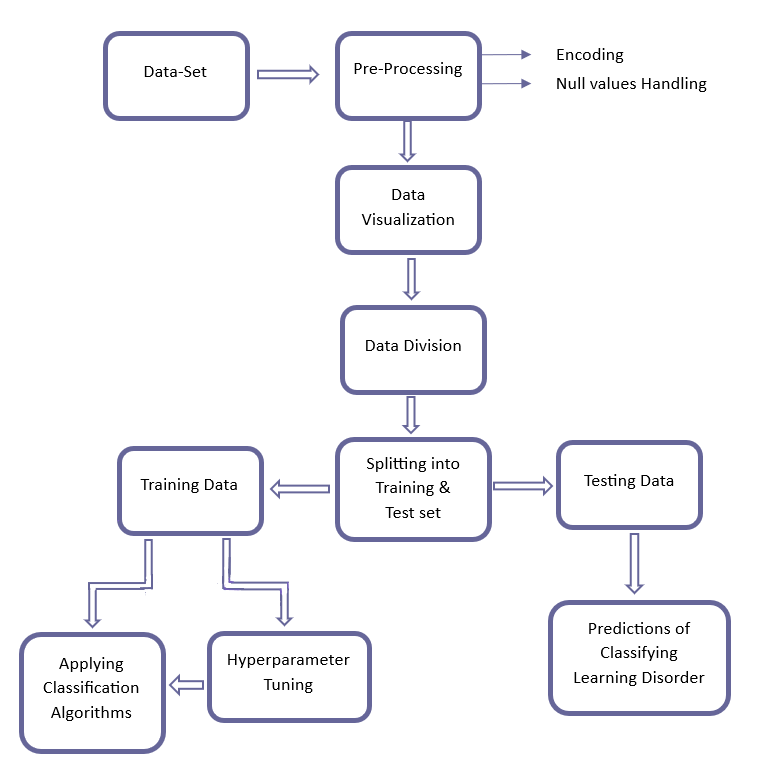
\includegraphics[width=1.05\textwidth]{images/map.png}
            \caption{Methodology of the work}
            \vspace{0.1em}
            \label{mapping}
        \end{figure}
    \end{minipage}

\vspace{3\baselineskip}
\begin{multicols}{2}



\subsubsection{Converting categorical data to numerical representations}
\hspace*{\parindent}In our dataset, we had several columns which composed of categorical values. The columns consisting categorical values are -- 
``Speech Delay/Language Disorder'', ``Learning disorder'', ``Genetic\_Disorders'', ``Depression'', ``Global developmental delay/Intellectual disability'', ``Sex'', ``Ethnicity'', ``Jaundice'', ``Childhood Autism Rating Scale'', ``Anxiety\_disorder'', ``Family\_mem\_with\_ASD'', ``Who\_completed\_the\_test'', ``ASD\_traits''.
So, we used label encoder on these categorical values and converted them to their respective numerical representations, so that machine learning algorithms can be applied to the whole dataset now too.

\subsection{Splitting the dataset}
\hspace*{\parindent}After data preprocessing was done completely, the resulting preprocessed dataset was split into train set and test set. The target column(y) was the ``Learning disorder'' column while the features(X) were all the remaining columns except ``CASE\_NO\_PATIENTS'' which was dropped since it was just the numerical representation of total rows in dataset and the ``Learning disorder'' column which is the target column. The dataset was then split in a 80-20 ratio where training set consists of 80\% data, and test set consists of 20\% data.

\subsection{Data Visualization}
    \hspace*{\parindent}Fig.~\ref{fig:gender-pie-chart} provides information on the percentage of children participants of the collected ASD dataset. About 72.9\% of the total participants were male whereas the rest 27.1\% were female. This was crucial for us as it give us the insights into the total number of participants and also the imbalance in the dataset.\\
    
    \noindent
    \hspace*{\parindent}Fig.~\ref{fig:gender-pie-chart-asd} shows the actual percentage of male (89.7\%) and female (10.3\%) children who possess the ASD trait. According to the pie chart male children are far more prone to being affected with ASD than female children.\\
    
    \noindent
    \hspace*{\parindent}Fig.~\ref{fig:age-bar-asd} demonstrates the distribution of age for all the participants in this dataset, which ranges from 1 to 18 inclusive. We can see here that the highest number of patients are of the age 14, consisting of about 316 children. This information here tells us that ASD is much more visible at that age point.\\
    \begin{minipage}{\columnwidth}
    \centering
        \begin{figure}[H]
            \begin{subfigure}{\columnwidth}
                \centering
                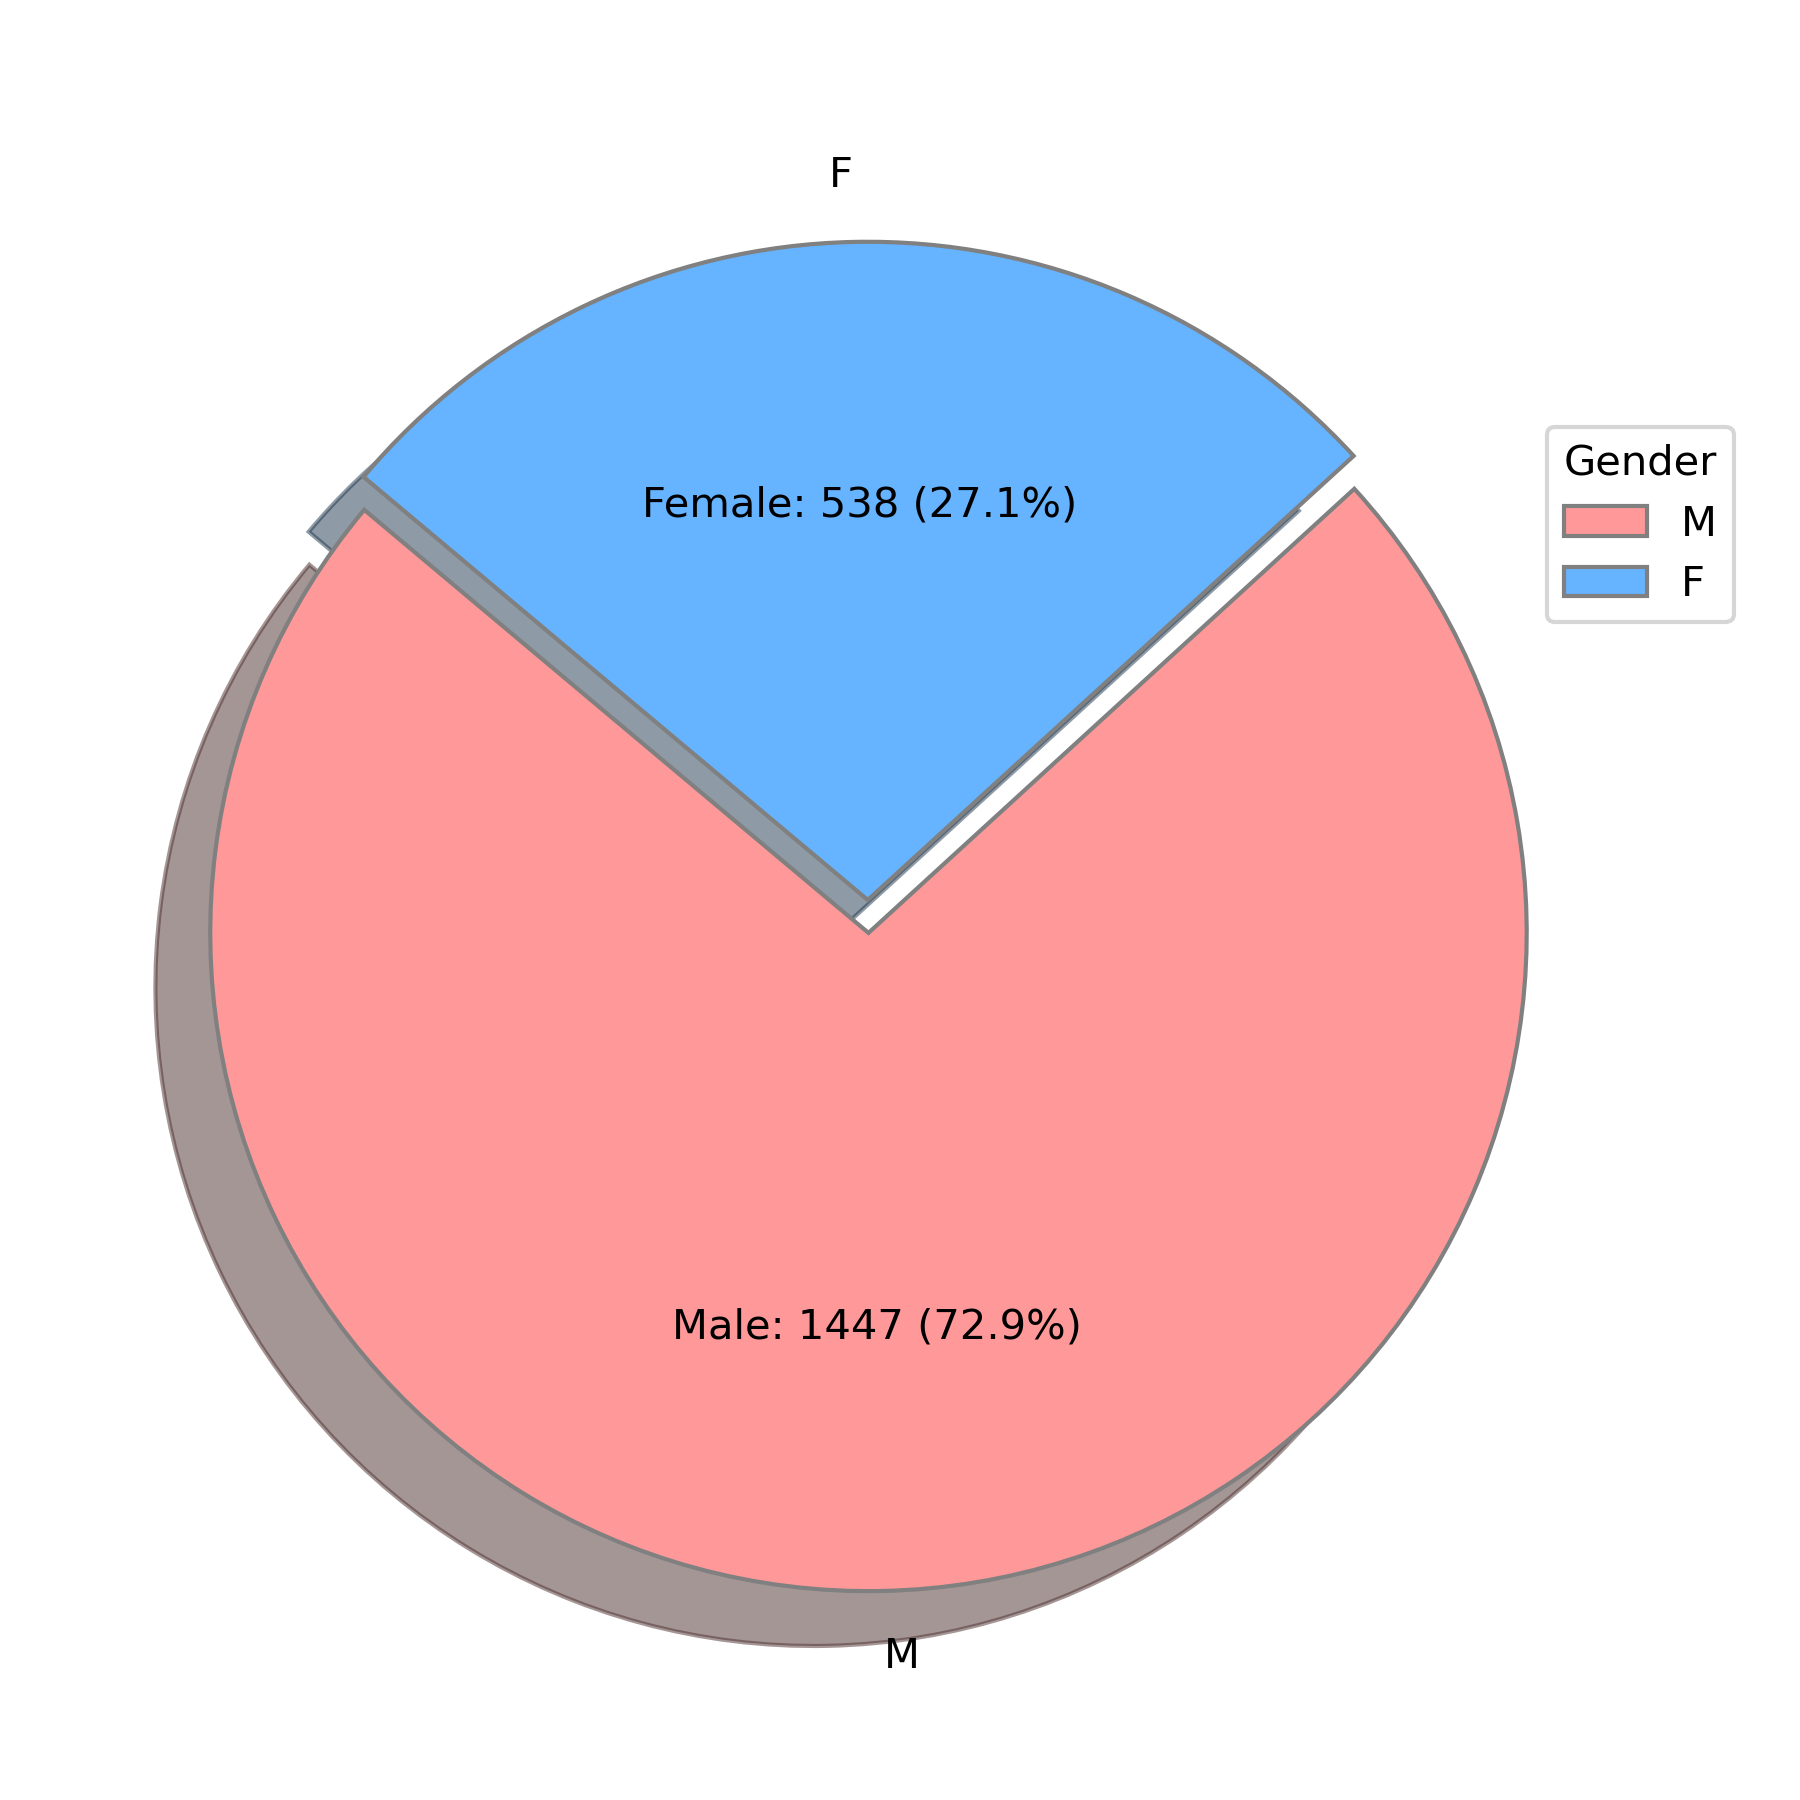
\includegraphics[width=\textwidth]{images/Gender_Pi_chart.png}
                \caption{}
                \label{fig:gender-pie-chart} % Add a label to reference the figure
            \end{subfigure}
            \hfill
            \begin{subfigure}{\columnwidth}
                \centering
                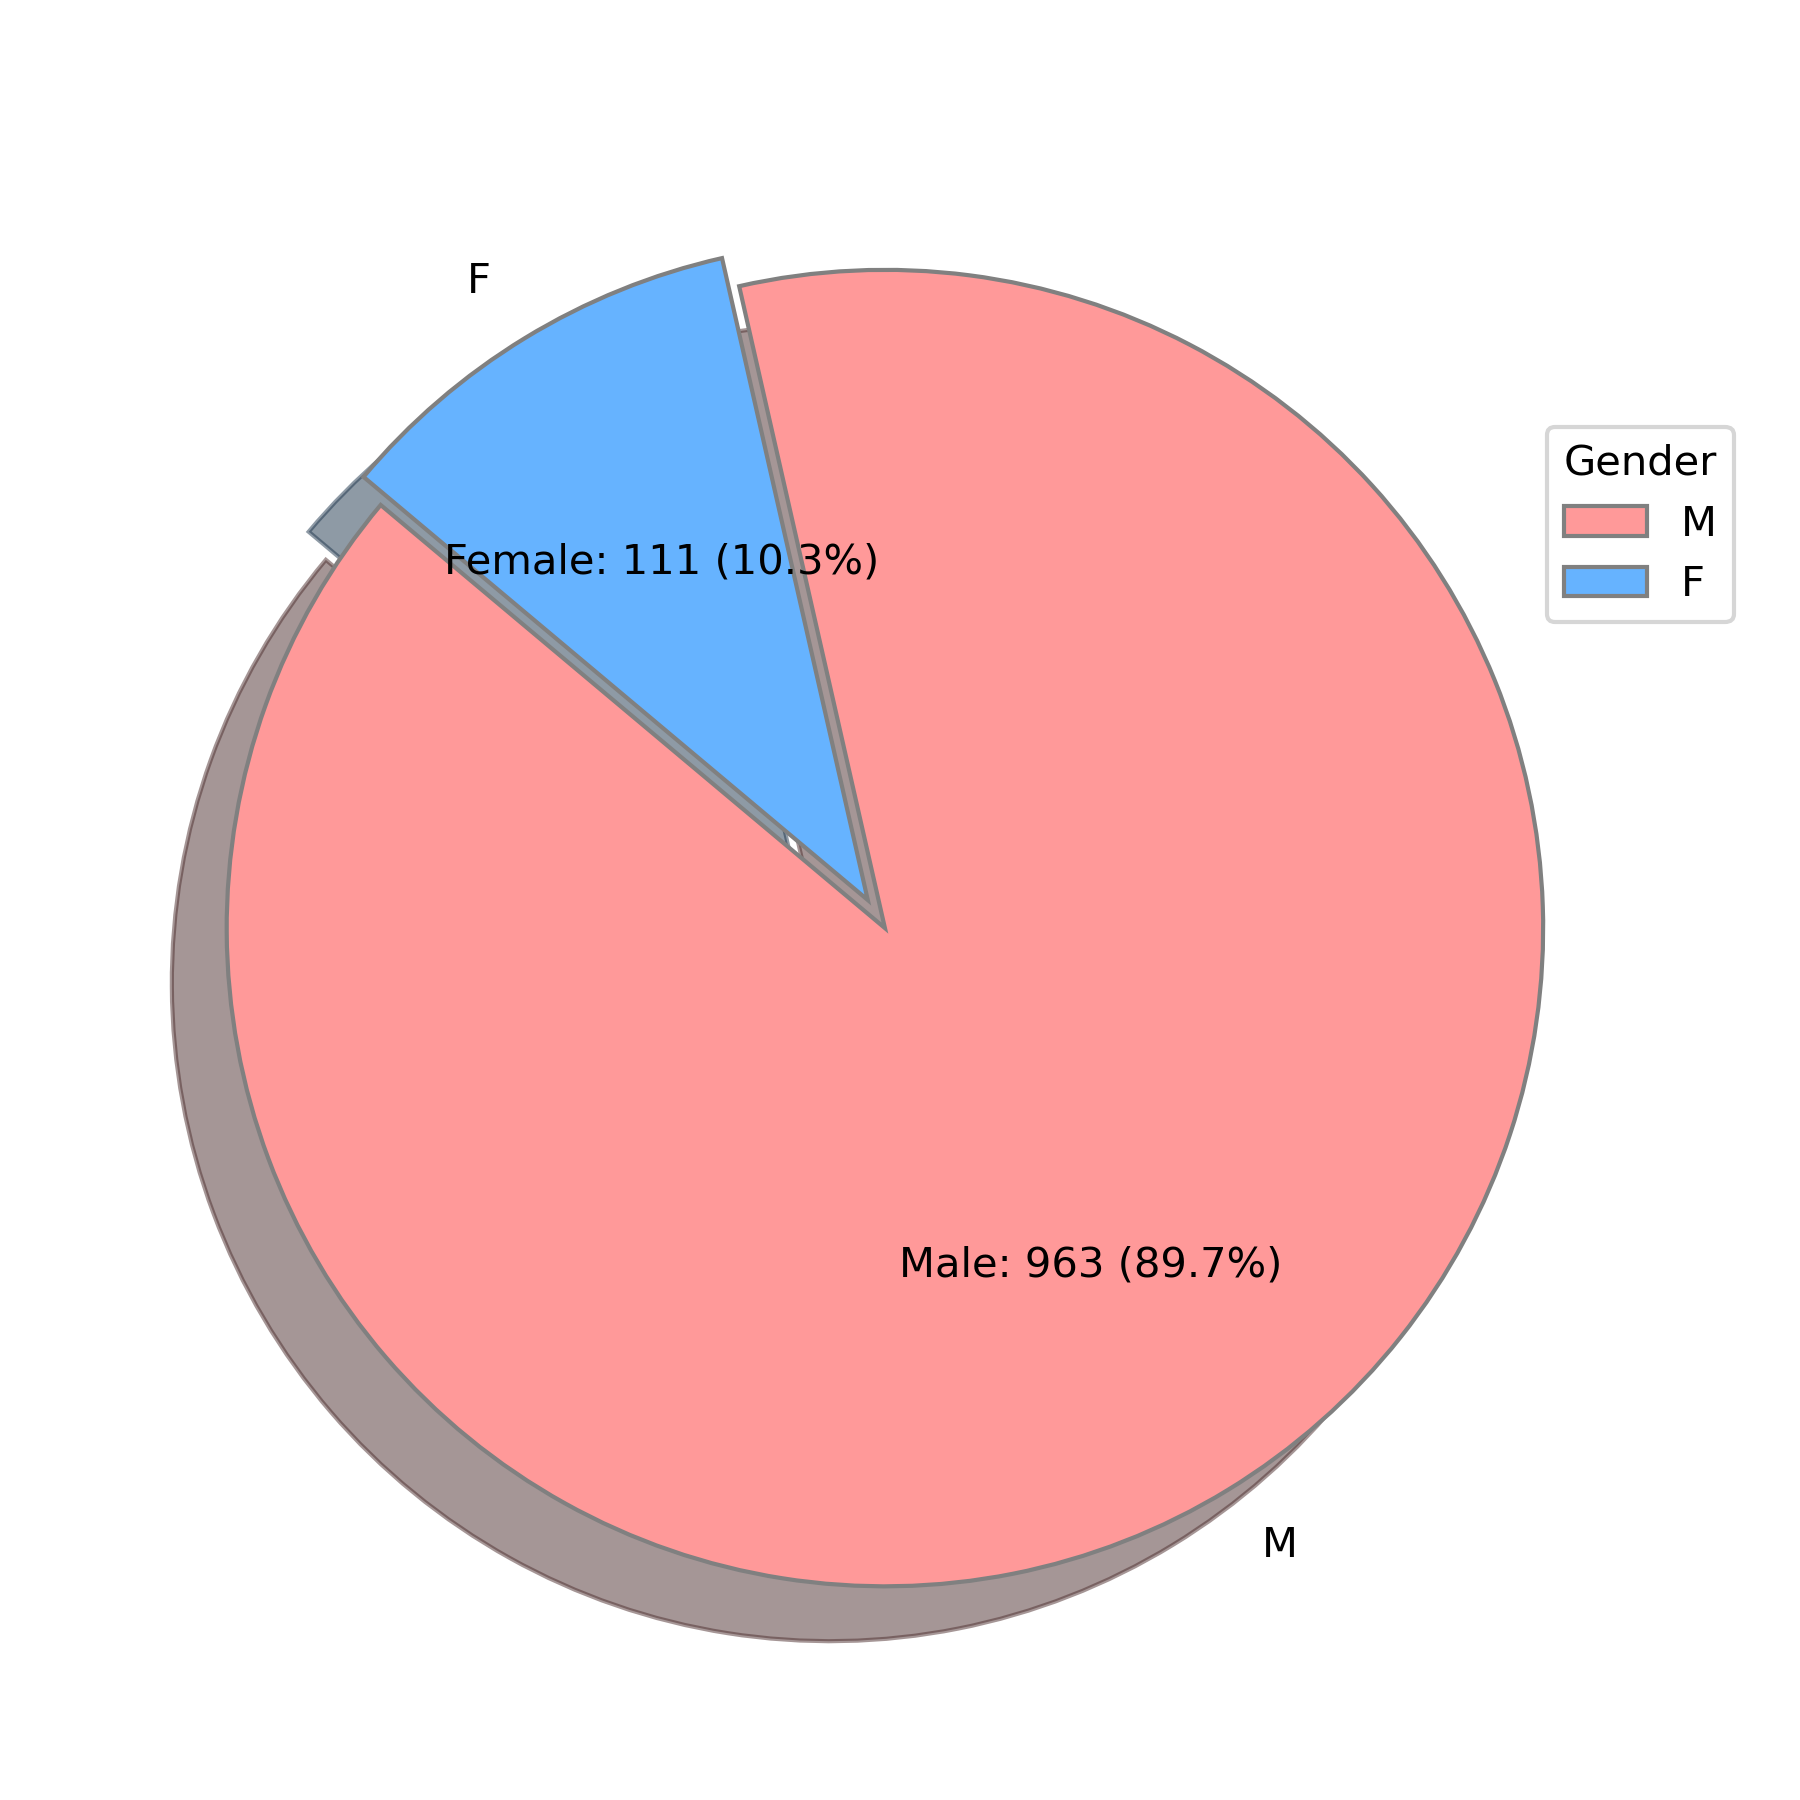
\includegraphics[width=\textwidth]{images/Gender_Pi_chart(asd).png}
                \caption{}
                \label{fig:gender-pie-chart-asd} % Add a label to reference the figure
            \end{subfigure}
            \caption{Percentage distribution of (a) participants, (b)participants with ASD grouped by gender }
            \label{fig:gender-distribution}
        \end{figure}
    \end{minipage}
    \vspace{1.2em}
    
    \noindent
    \hspace*{\parindent}Fig.~\ref{fig:Qchat-bar-asd} shows the Qchat 10 score of the participants for this research. Qchat 10 score is a quantitative checklist for autism in toddlers. There are 10 questions, and based on the answers and accumulating the scores, if the score is more than 3, they are referred for multi-disciplinary assessment.\\
    \end{multicols}
    
    \noindent
    \begin{figure}[H]
        \centering
        \fbox{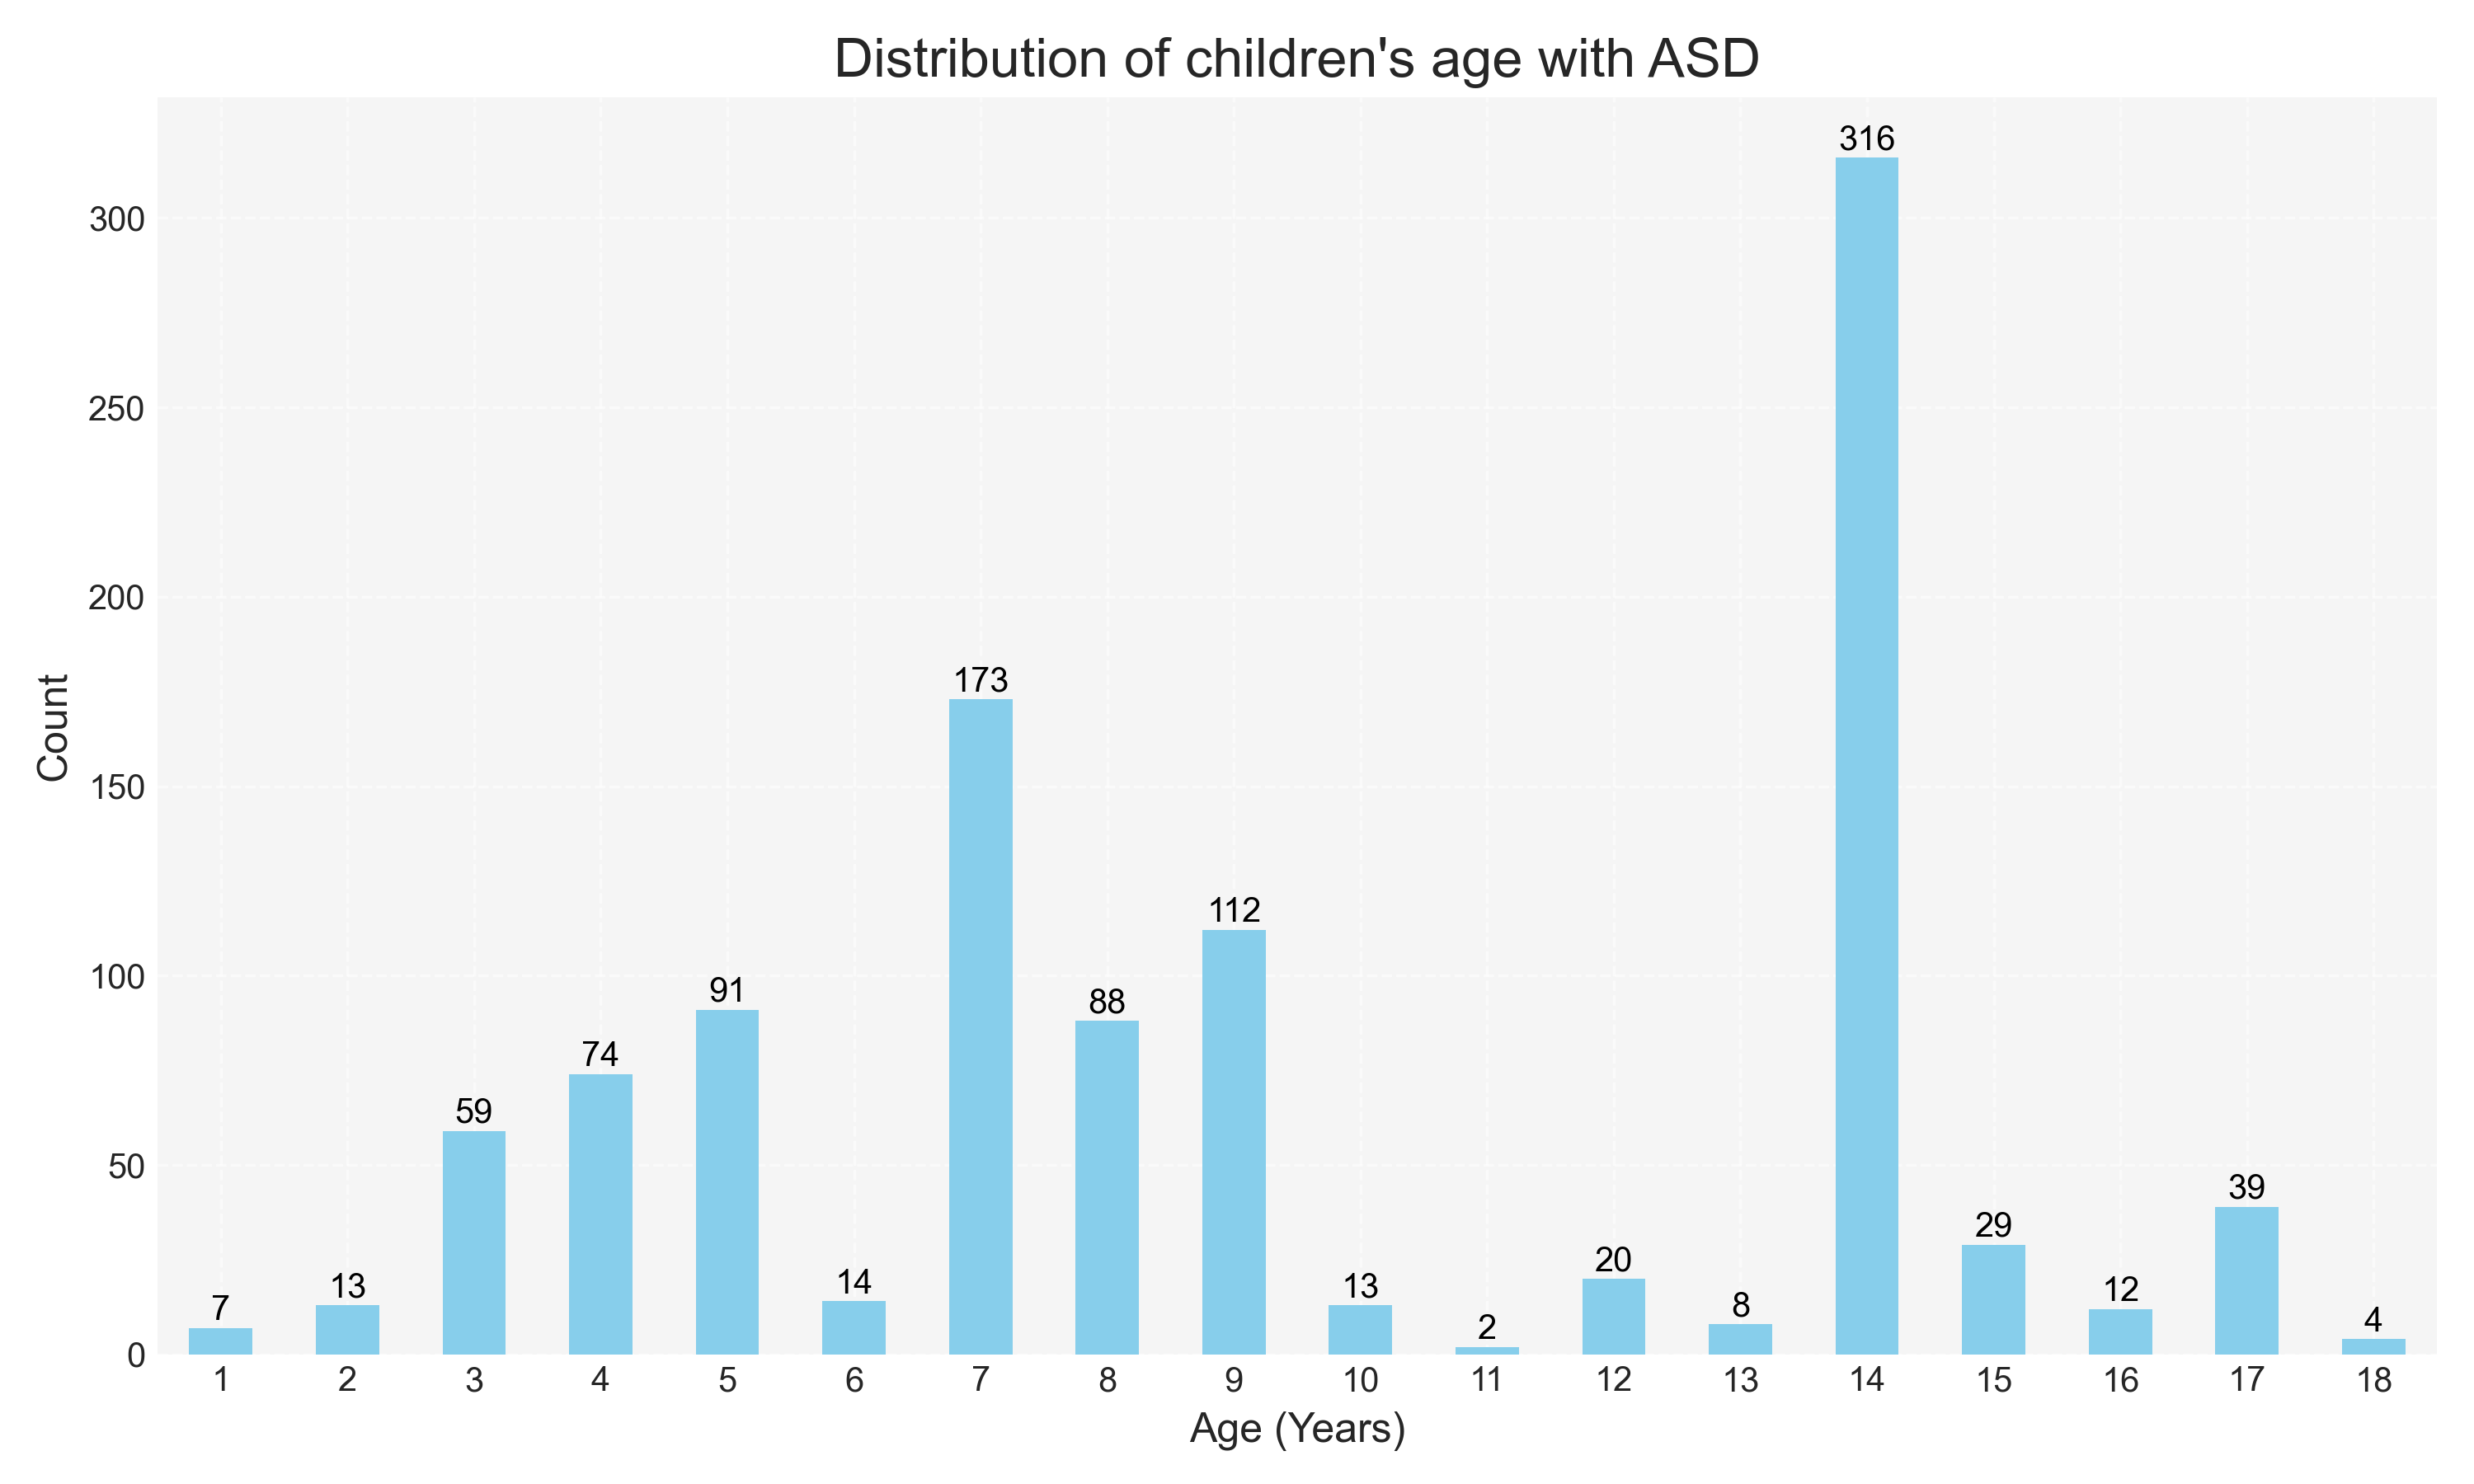
\includegraphics[width=\textwidth, height=225px]{images/Age_in_years_Bar_chart(asd).png}}
        \caption{Distribution of children with ASD}
        \vspace{1em}
        \label{fig:age-bar-asd}
    \end{figure}
    \begin{figure}[H]
        \centering
        \fbox{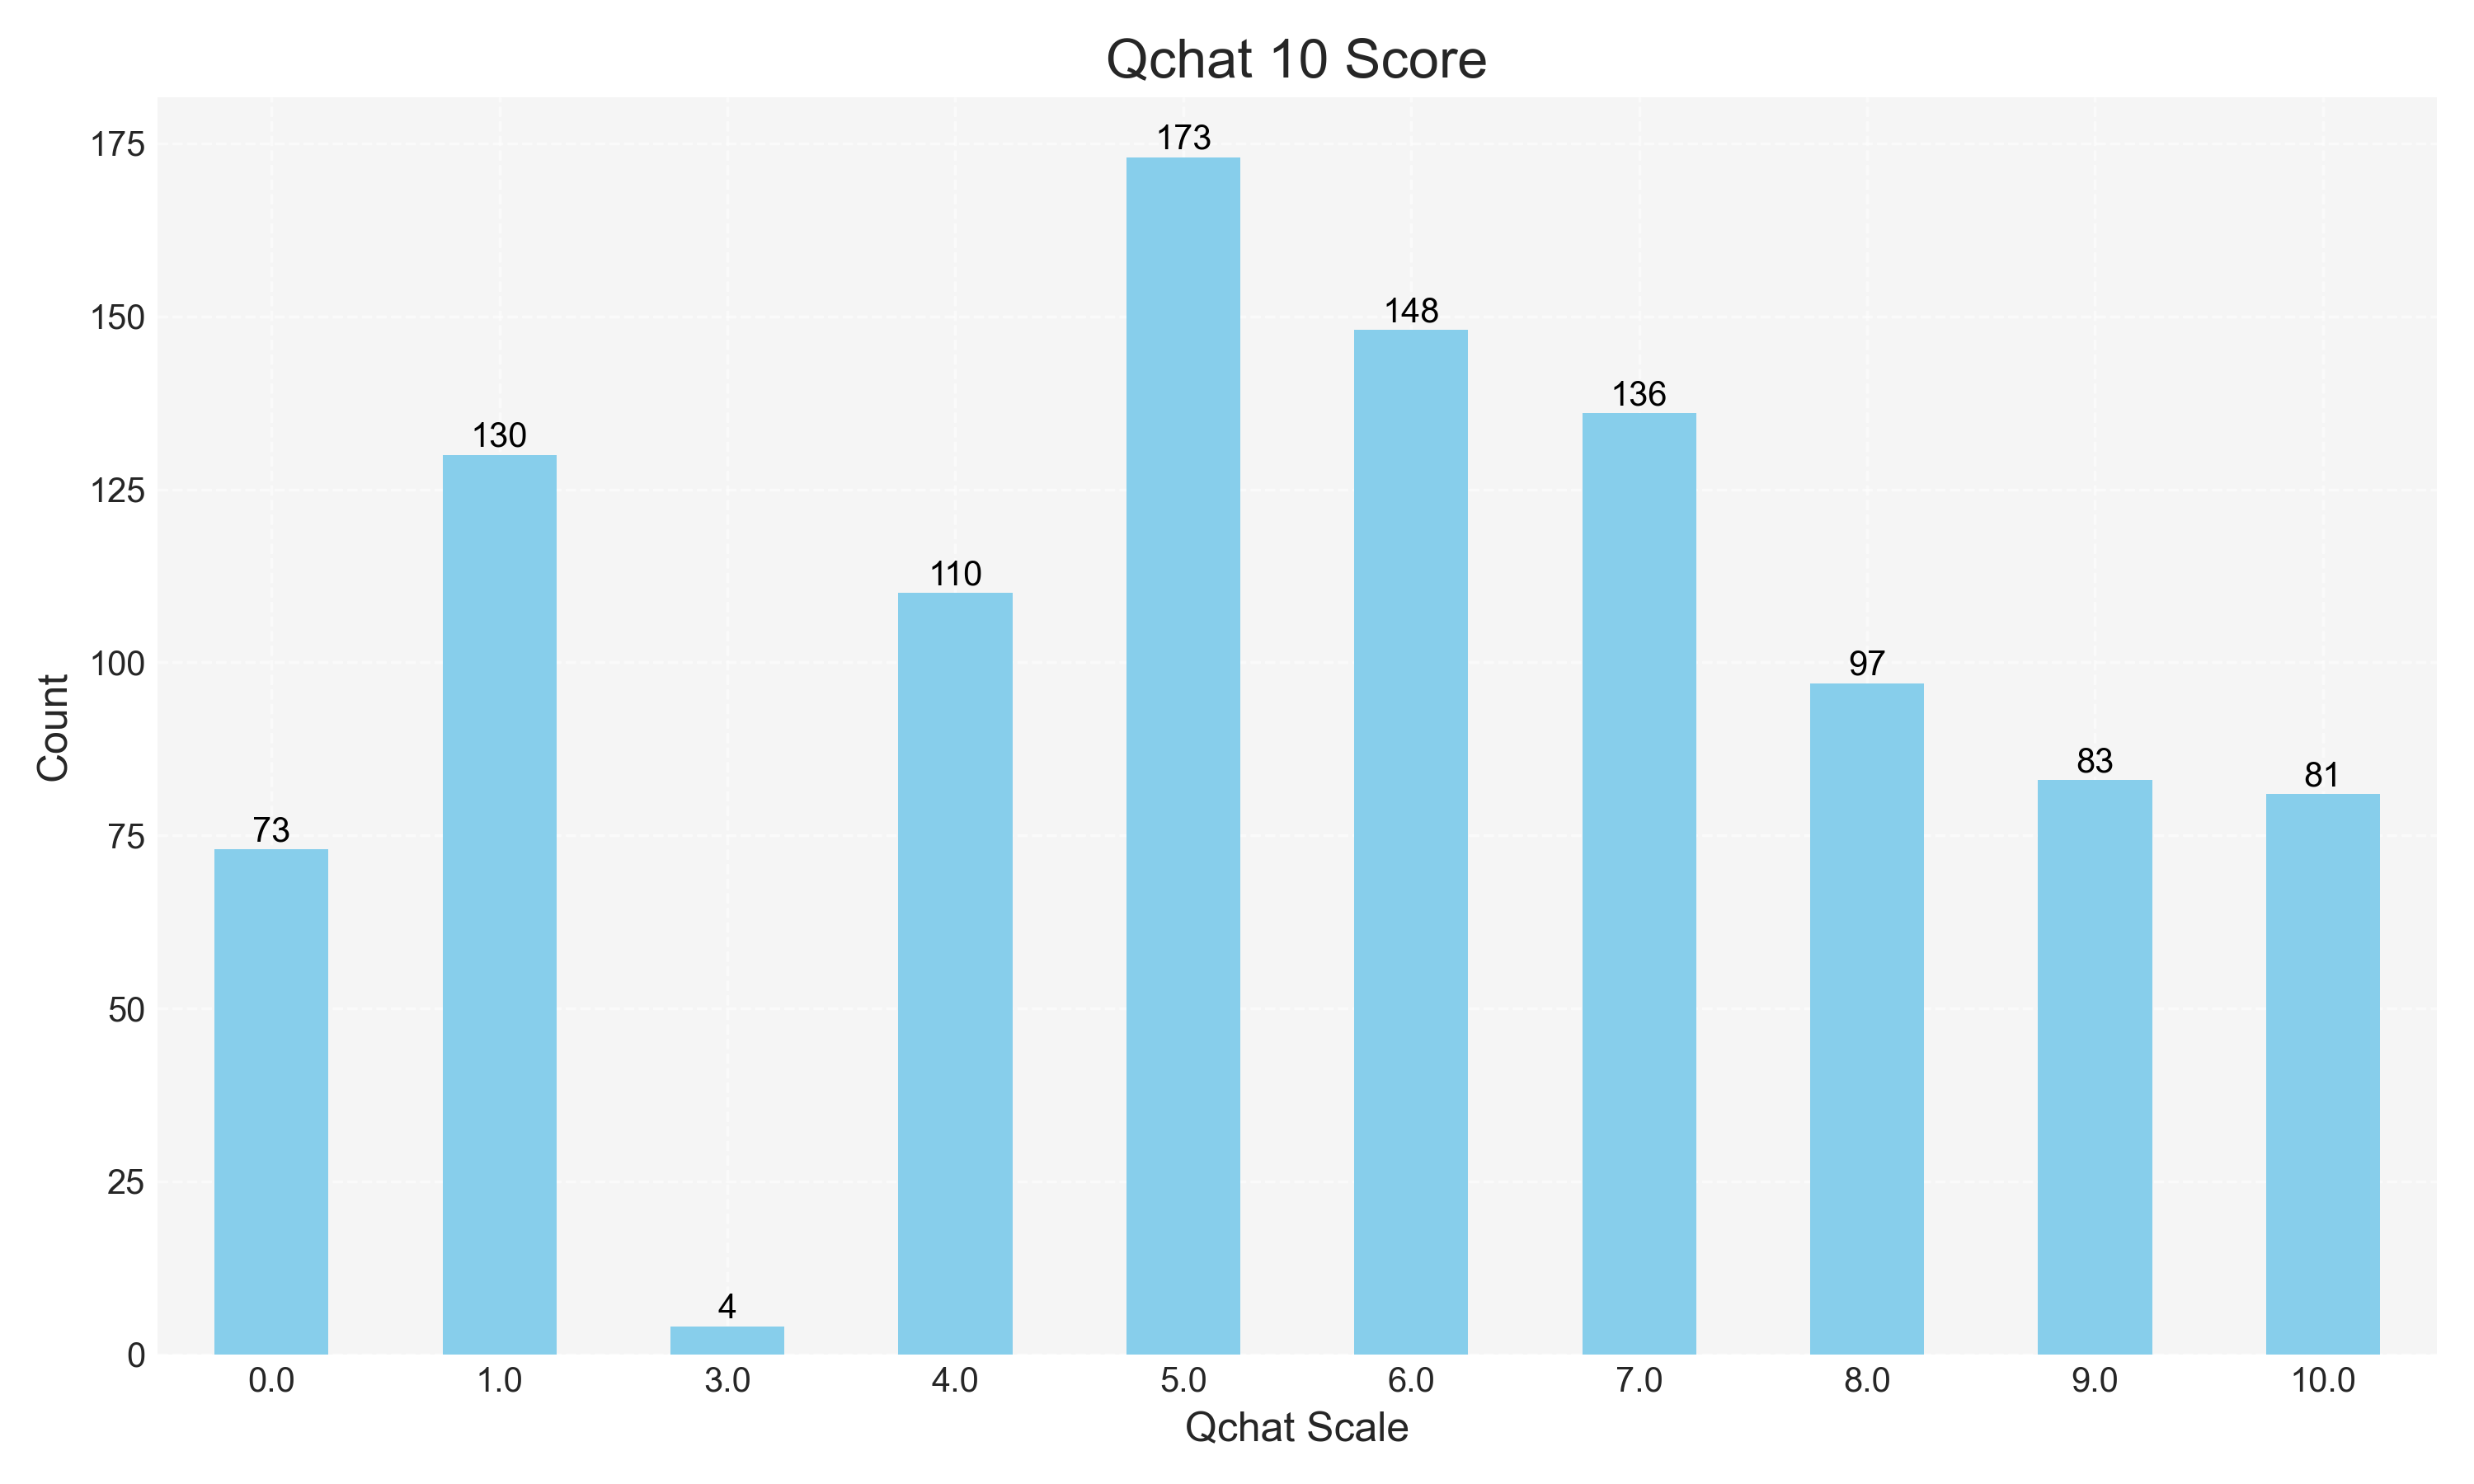
\includegraphics[width=\textwidth, height=225px]{images/Qchat 10 Score(asd).png}}
        \caption{QChat 10 score of children with ASD}
        % \vspace{1em}
        \label{fig:Qchat-bar-asd}
    \end{figure}

    \begin{multicols}{2}
    \noindent
    \hspace*{\parindent}Fig.~\ref{fig:depression-bar} shows how many participants suffer from depression given that they have ASD. It seems that twice as much participants who has ASD, suffer from depression.\\
    
    \noindent
    \hspace*{\parindent}Fig.~\ref{fig:anxiety-bar} shows how many of the participants have anxiety disorder among the participants. Anxiety disorder is a very common trait for any ASD patient. But the data shows that it might not be the case as most of them might have anxiety disorder but the number of not having that issue is also not less.\\
    
    \noindent
    \hspace*{\parindent}Fig.~\ref{fig:fam-with-asd} describes the number of participants with ASD who also has a family member with ASD. It seems it is balanced in this case.\\
    
    \noindent
    \hspace*{\parindent}Fig.~\ref{fig:learning-disorder} elaborates the number of participants with ASD suffering from learning disorders. For patients with ASD, it is a very common case that they have a learning disability which may take a lot of time to heal, and this prevalence of learning disorder in children with ASD traits is what we will be measuring thorugh our study.\\
    
    \noindent
    \hspace*{\parindent}Fig.~\ref{fig:ethnicity-pie} shows the vast diversity of ethnicity in the collected data of the dataset. Huge portion of the participants are White-Europeans, then the next majority are Asians then Middle Easterners and so on. This was not much, but it can be used later to measure the compatibility of the dataset collected from other parts of the world.\\
    
    \noindent
    \hspace*{\parindent}Fig.\ref{fig:social-response} represents the score given to the participants in regard to social responsiveness. It seems most of the participants refuse to make any social contact. It is worth noting there were lots of babies ranging from 1 to 3 years in it, they are omitted for the sake of our research.\\

\end{multicols}
    
    \noindent
    \vspace{3em}
        \begin{figure}[H]
            \begin{subfigure}{0.45\textwidth}
                \centering
                \fbox{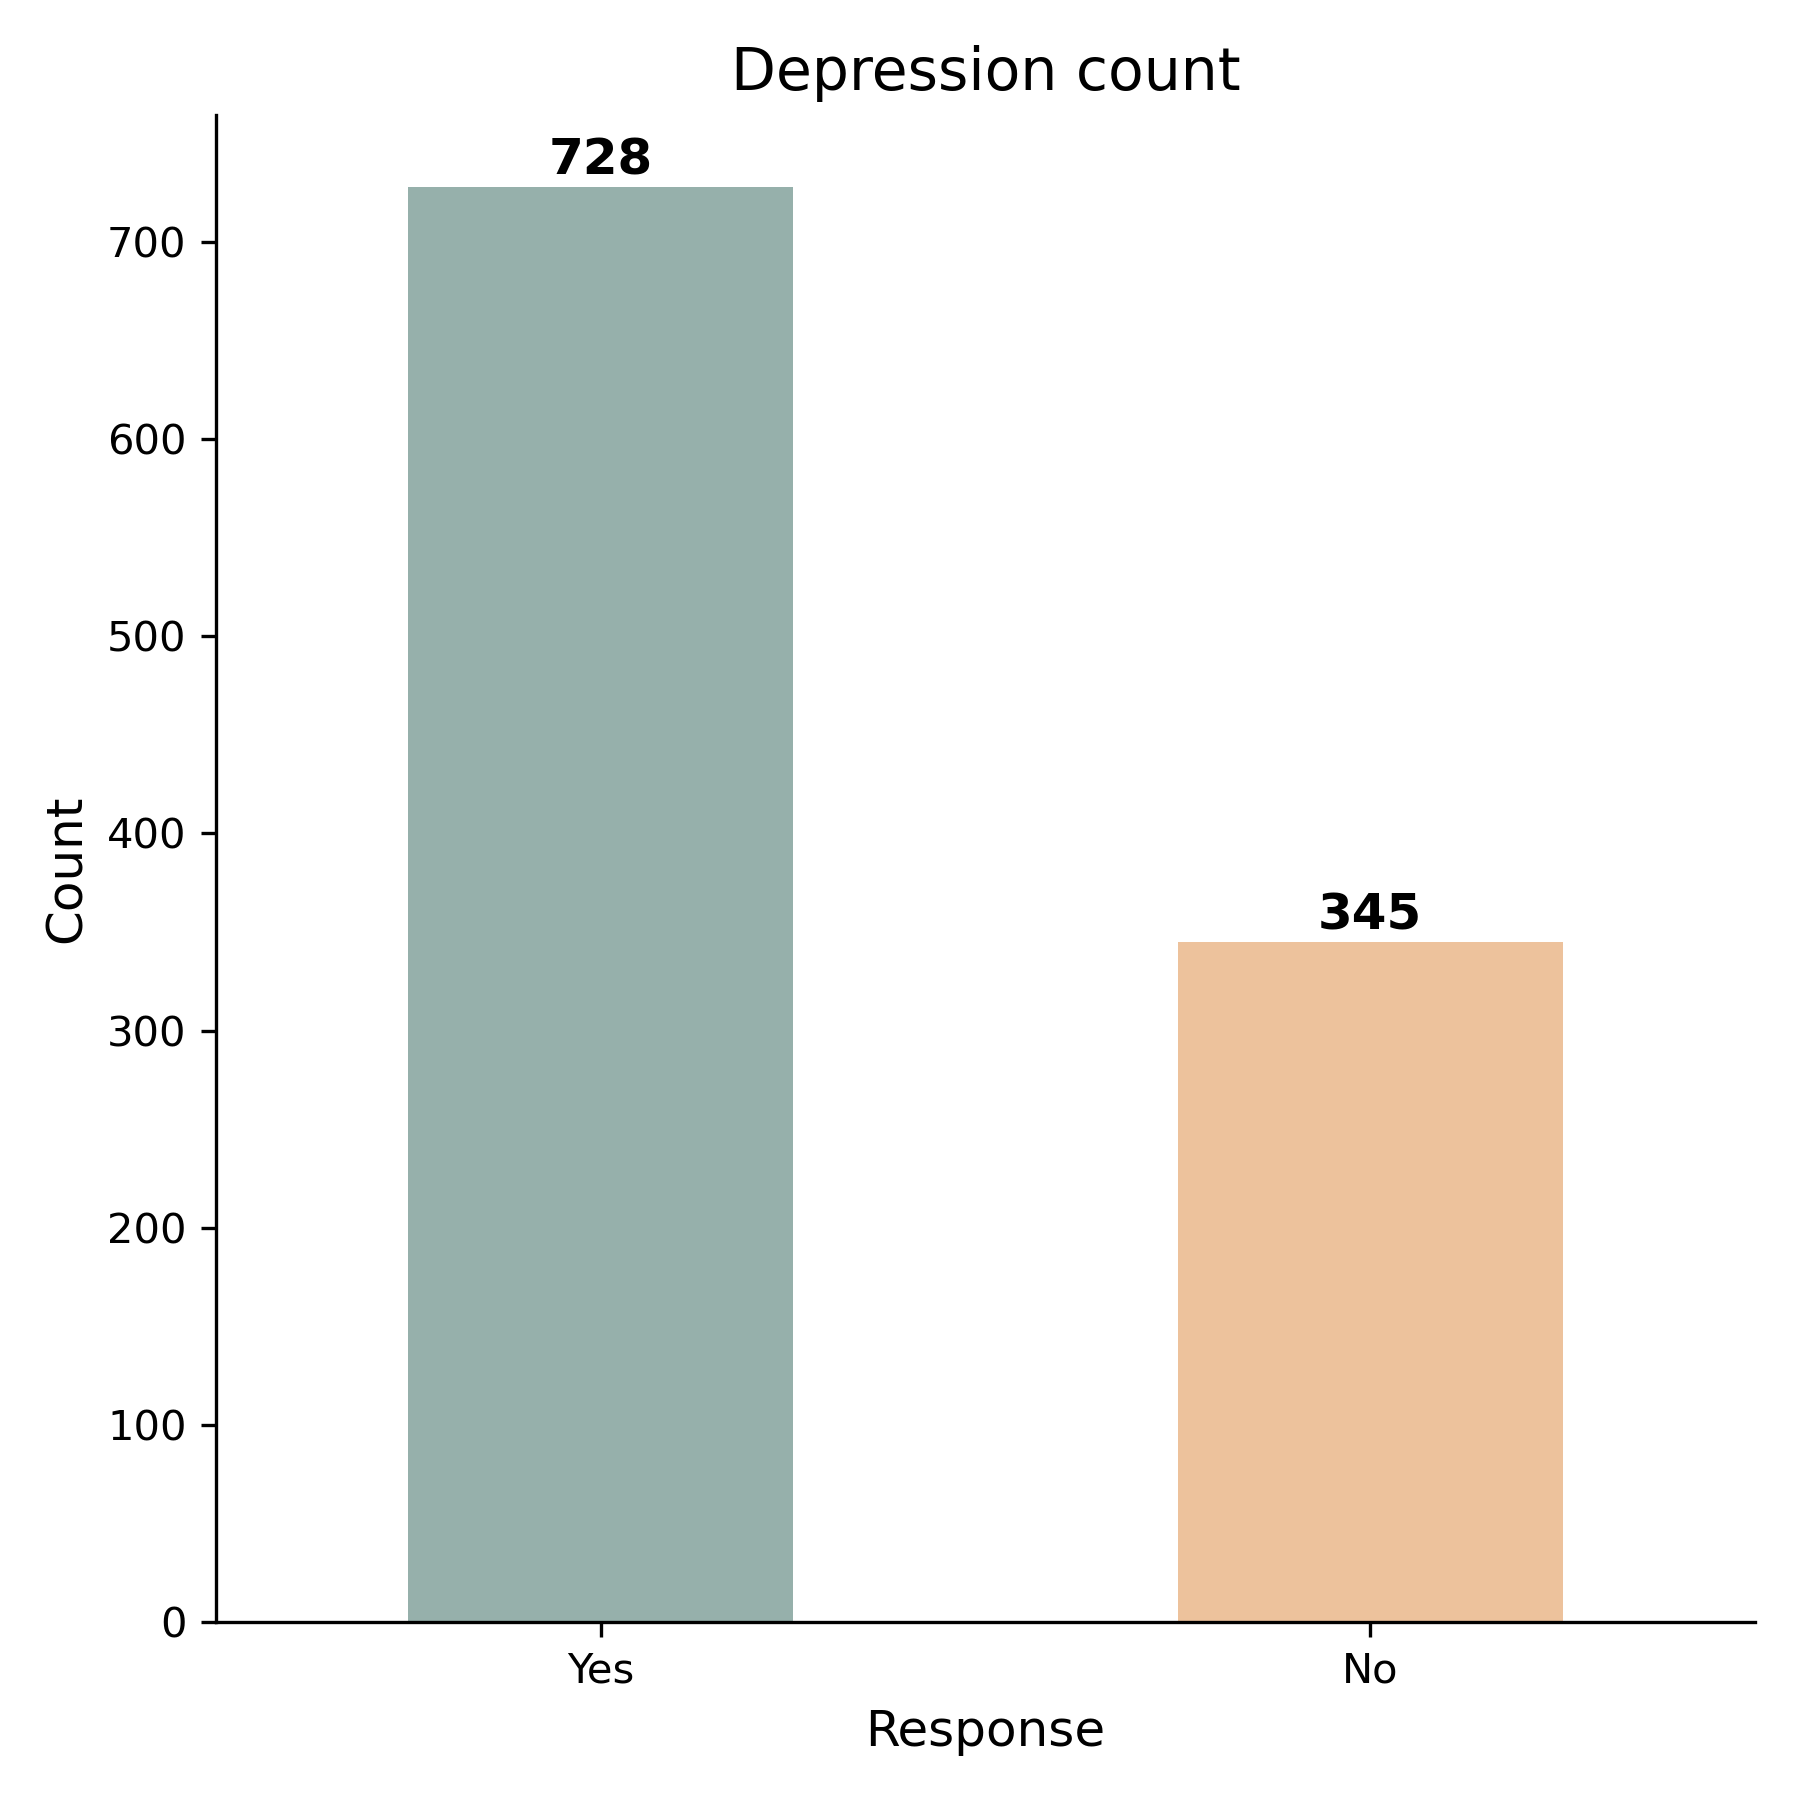
\includegraphics[width=\textwidth]{images/Depression bar(asd).png}}
                \caption{Participants with ASD suffering from depression}
                \vspace{1em}
                \label{fig:depression-bar}
            \end{subfigure}
            \hfill
            \begin{subfigure}{0.45\textwidth}
                \centering
                \fbox{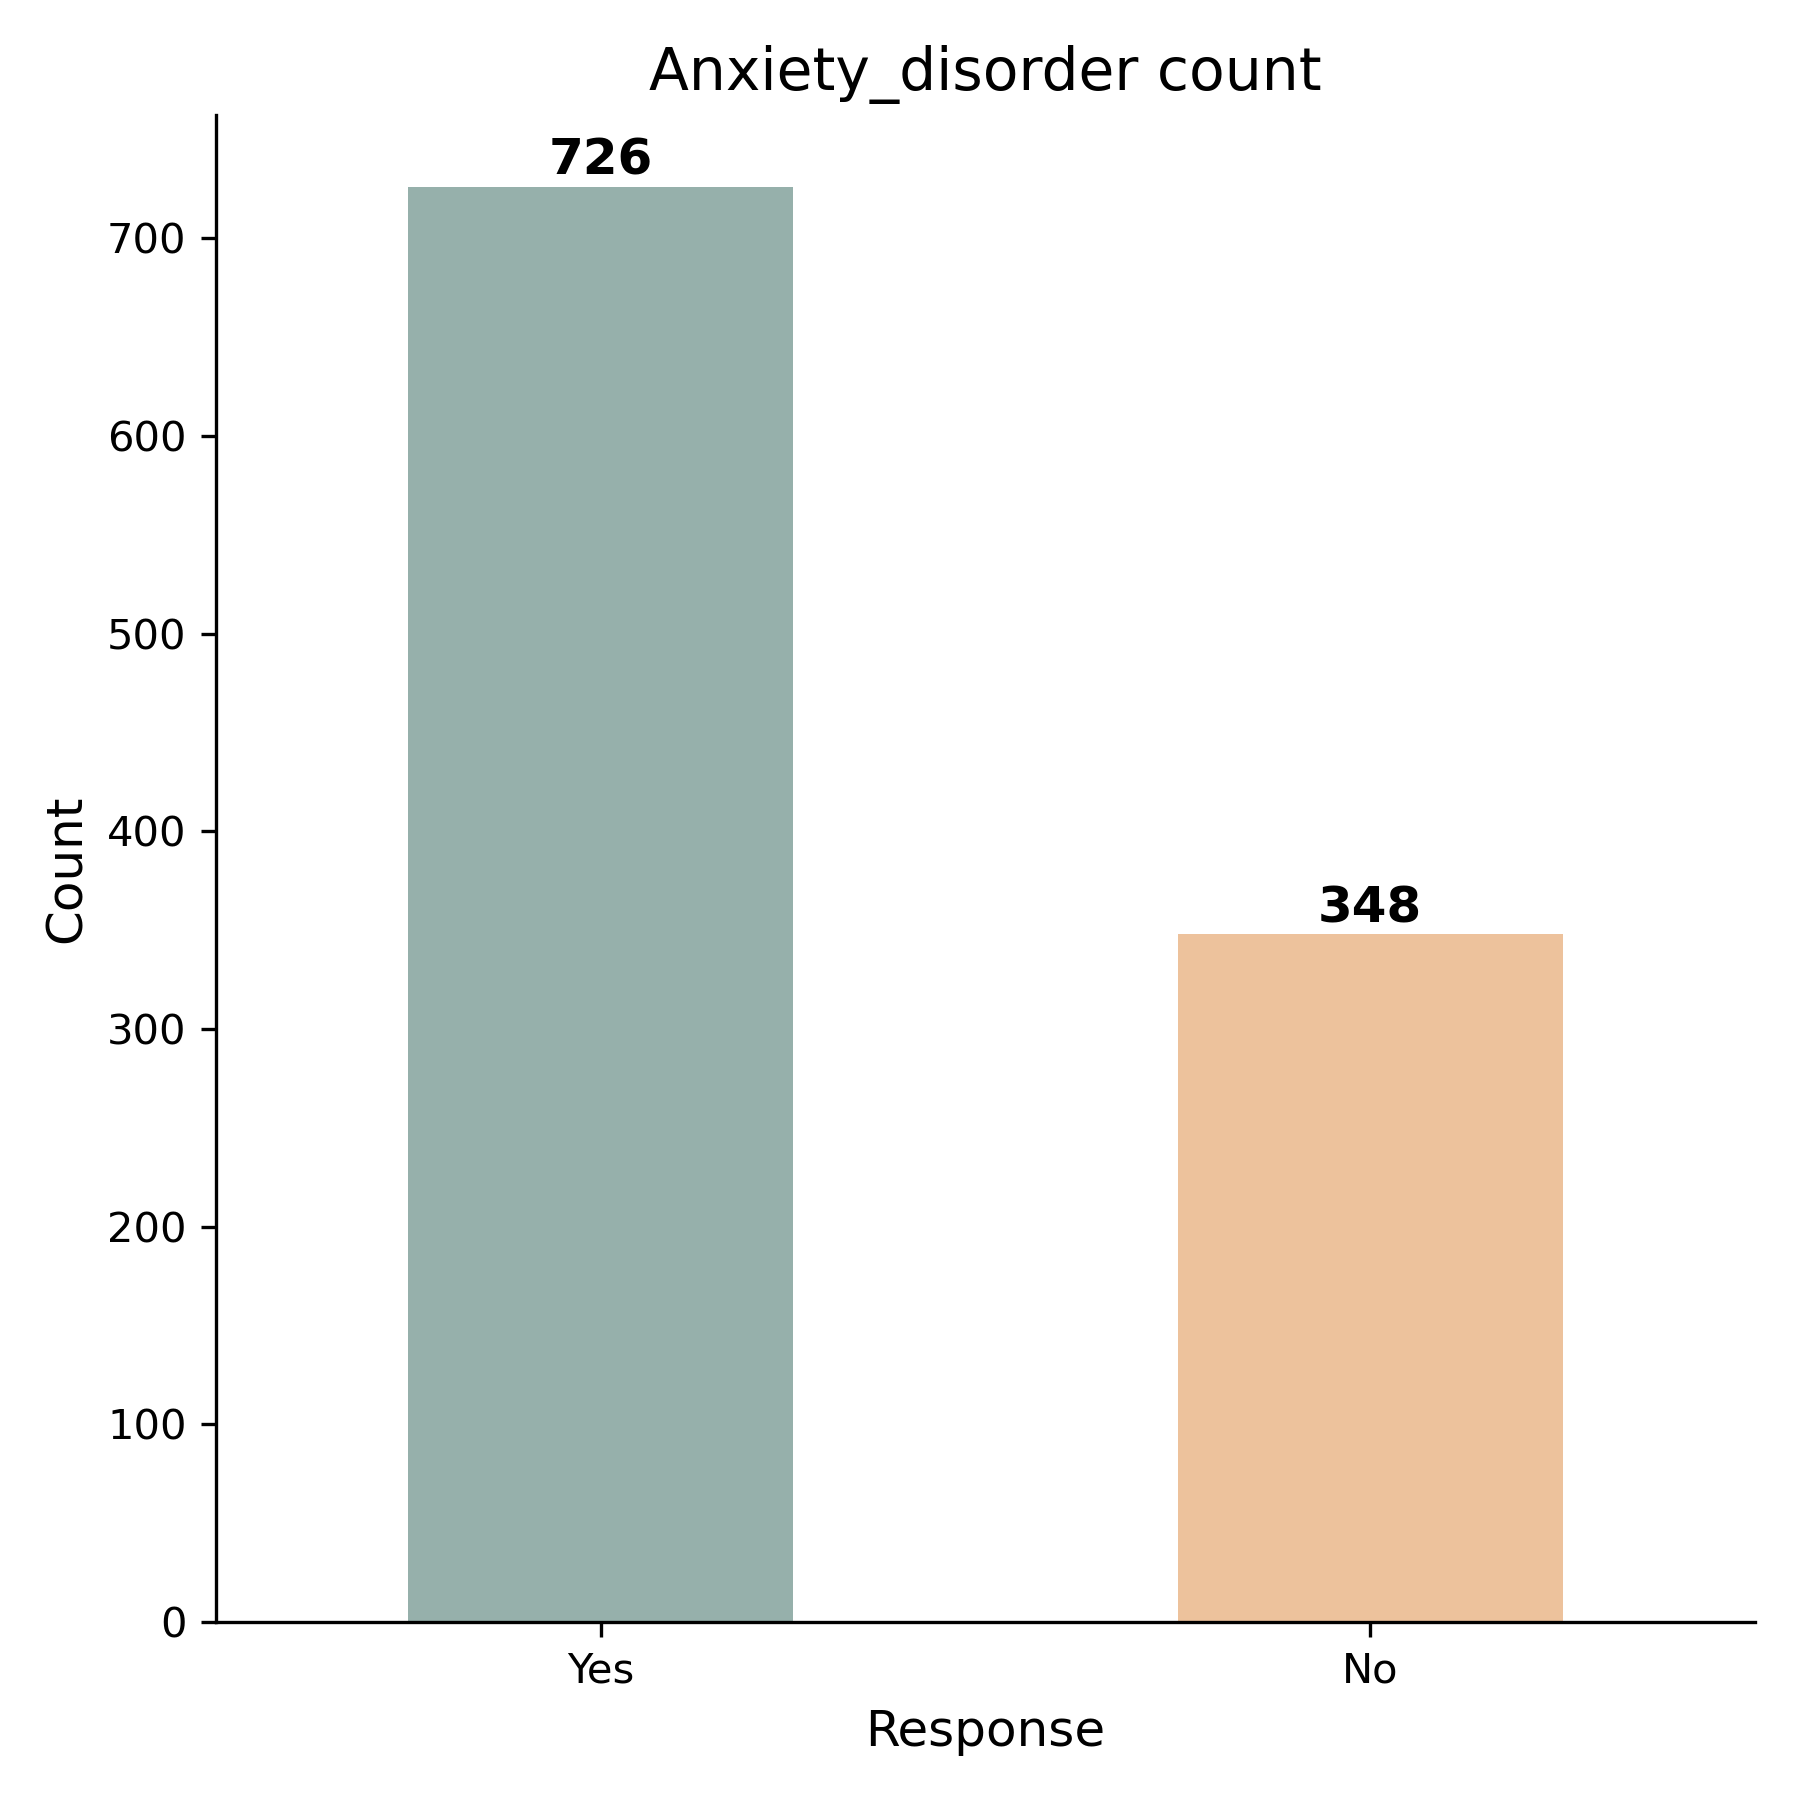
\includegraphics[width=\textwidth]{images/Anxiety_disorder bar.png}}
                \caption{Participants with ASD having anxiety disorder}
                \vspace{1em}
                \label{fig:anxiety-bar}
            \end{subfigure}
            \caption{Participants with ASD suffering from multiple disorders}
        \end{figure}
        
        \begin{figure}[H]
            \begin{subfigure}{0.45\textwidth}
                \centering
                \fbox{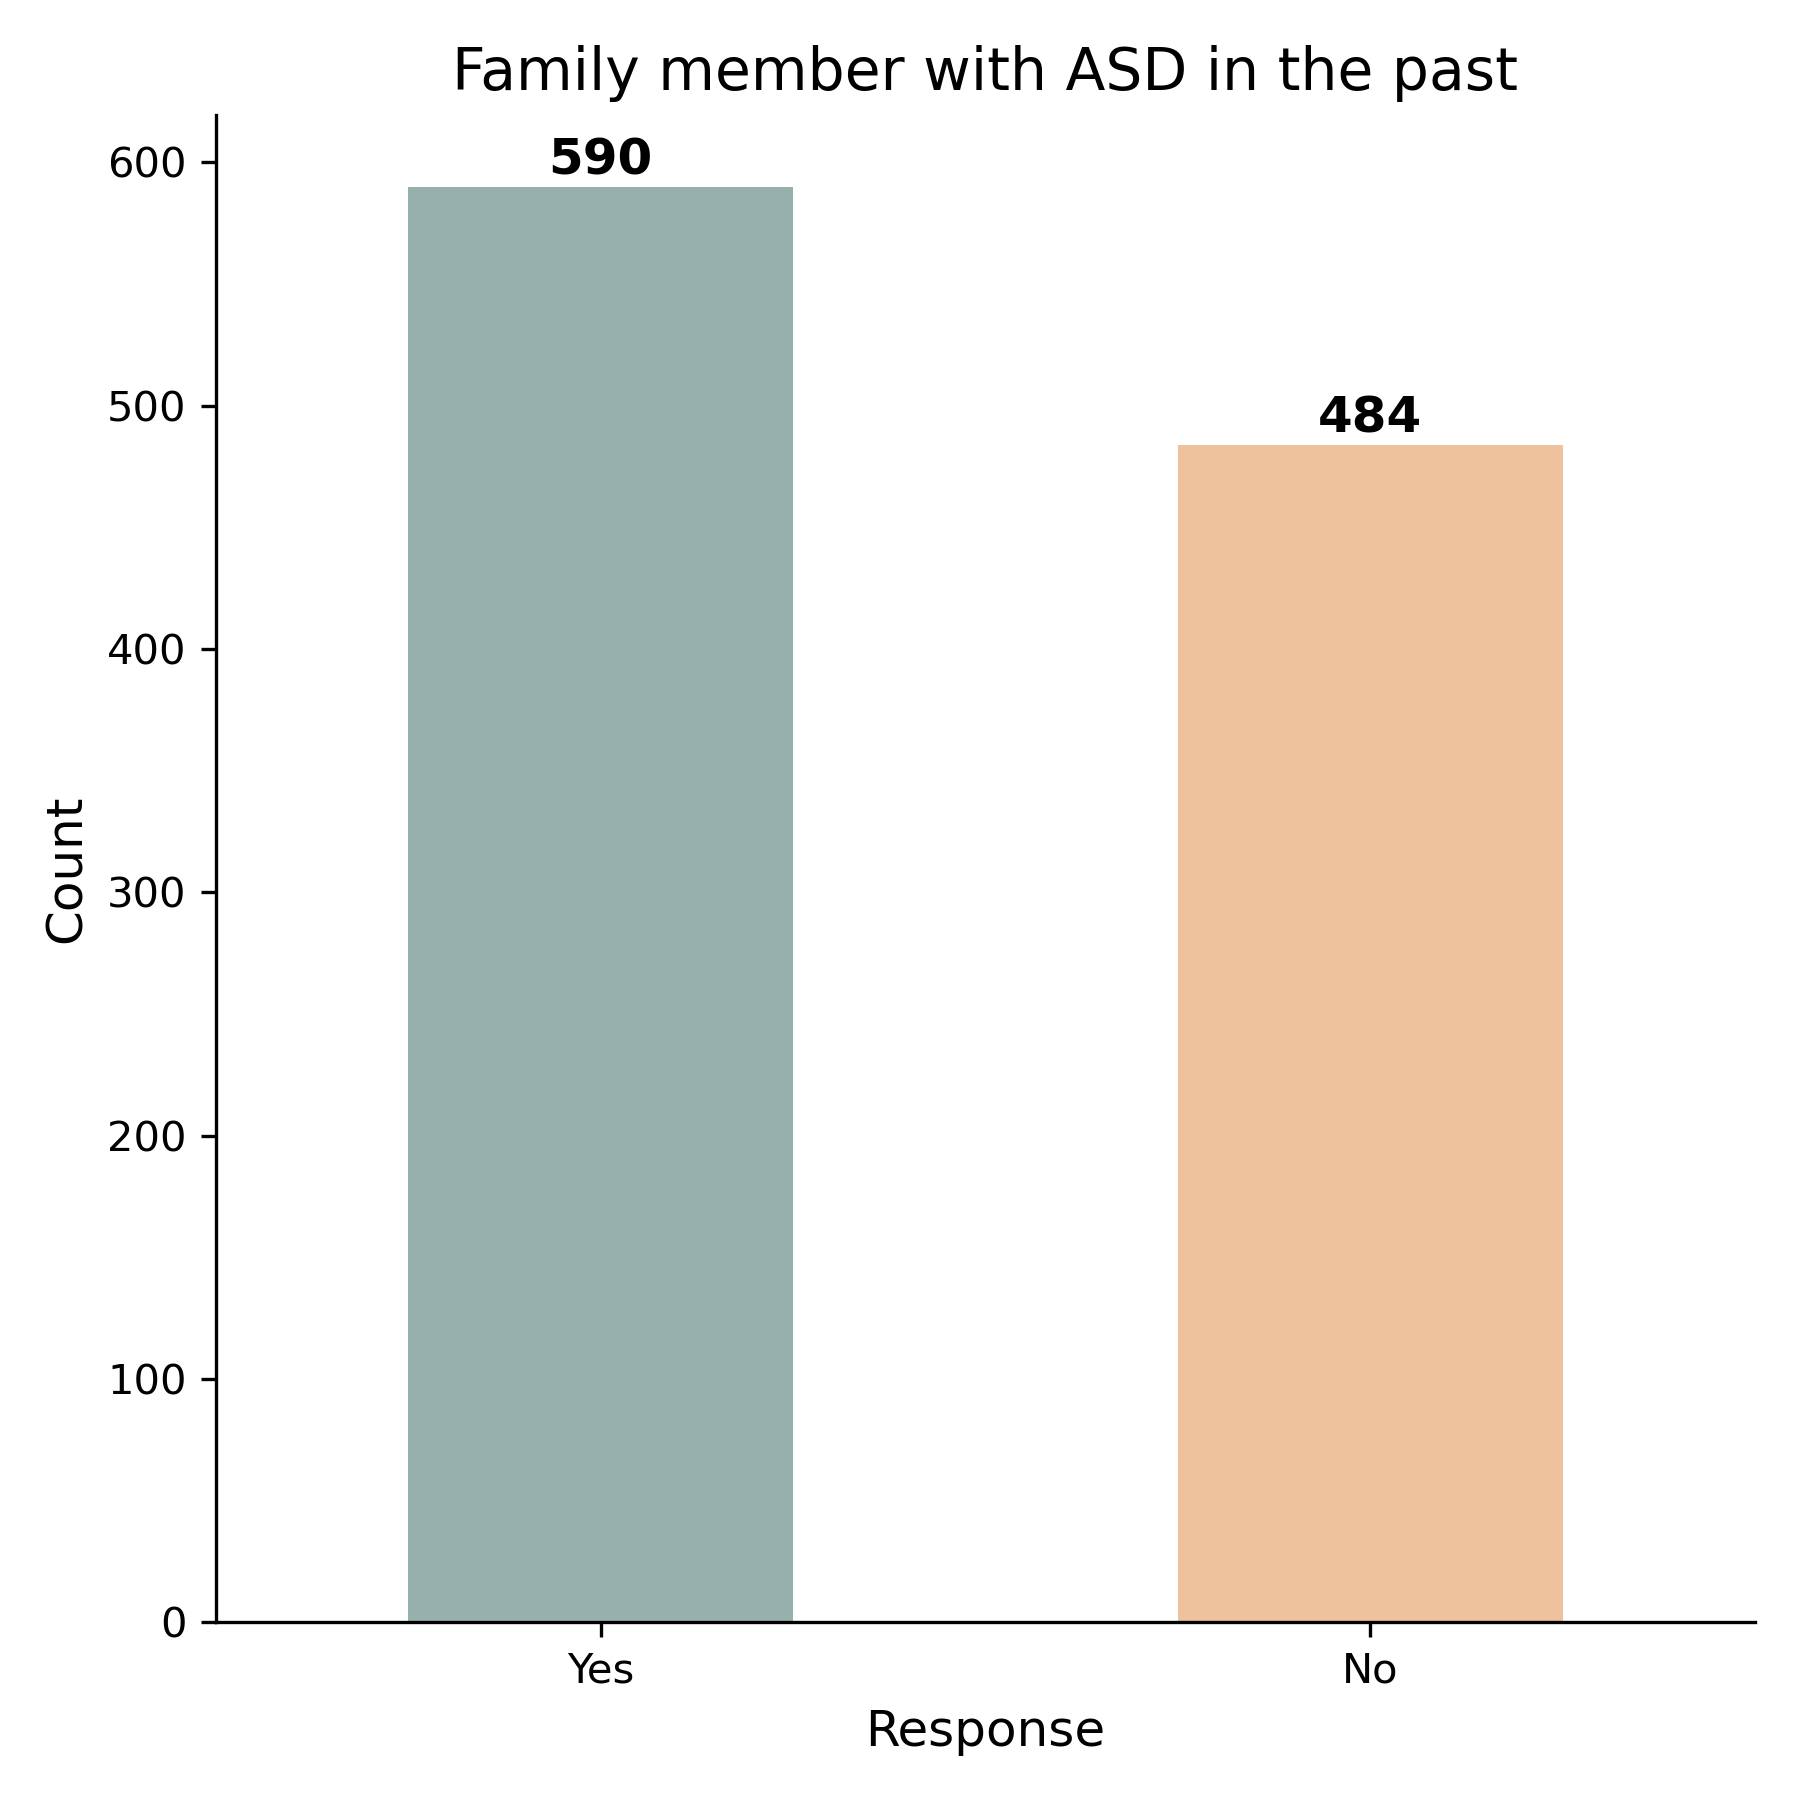
\includegraphics[width=\textwidth]{images/Family_with_asd_bar(asd).png}}
                \caption{Participants with ASD having another family member with ASD}
                \vspace{1em}
                \label{fig:fam-with-asd}
            \end{subfigure}
            \hfill
            \begin{subfigure}{0.45\textwidth}
                \centering
                \fbox{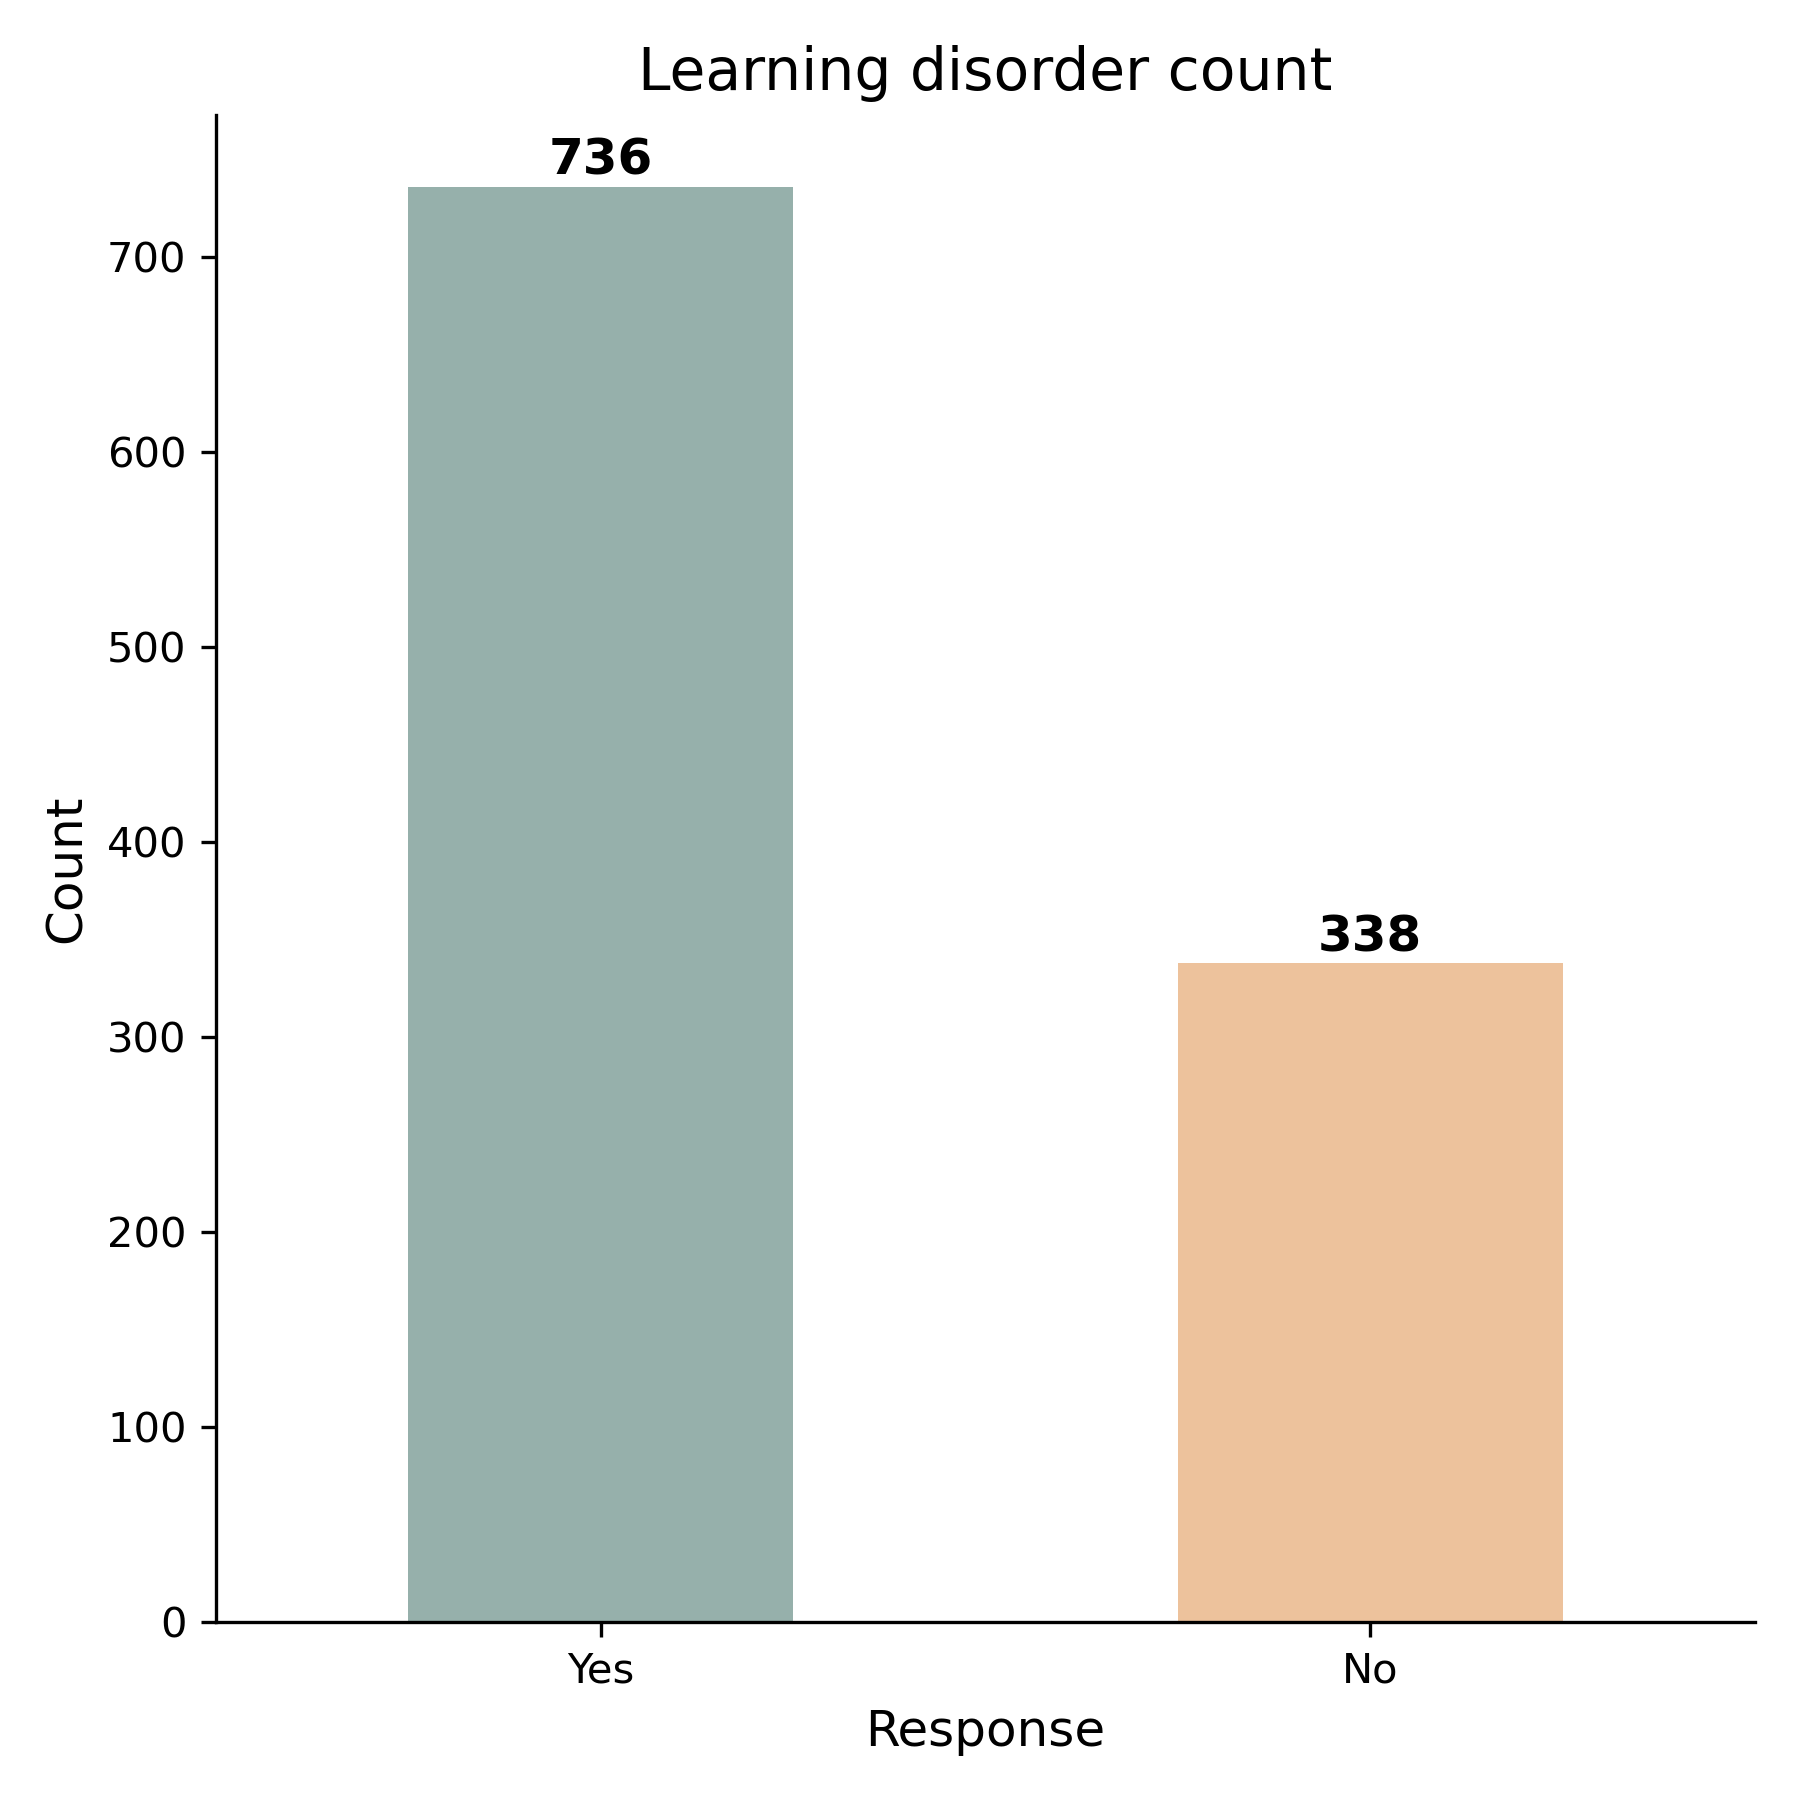
\includegraphics[width=\textwidth]{images/Learning disorder bar(asd).png}}
                \caption{Participants with ASD experiencing learning disorder}
                \vspace{1em}
                \label{fig:learning-disorder}
            \end{subfigure}
            \hspace*{7.6em}
            \begin{subfigure}{0.65\textwidth}
                \centering
                \fbox{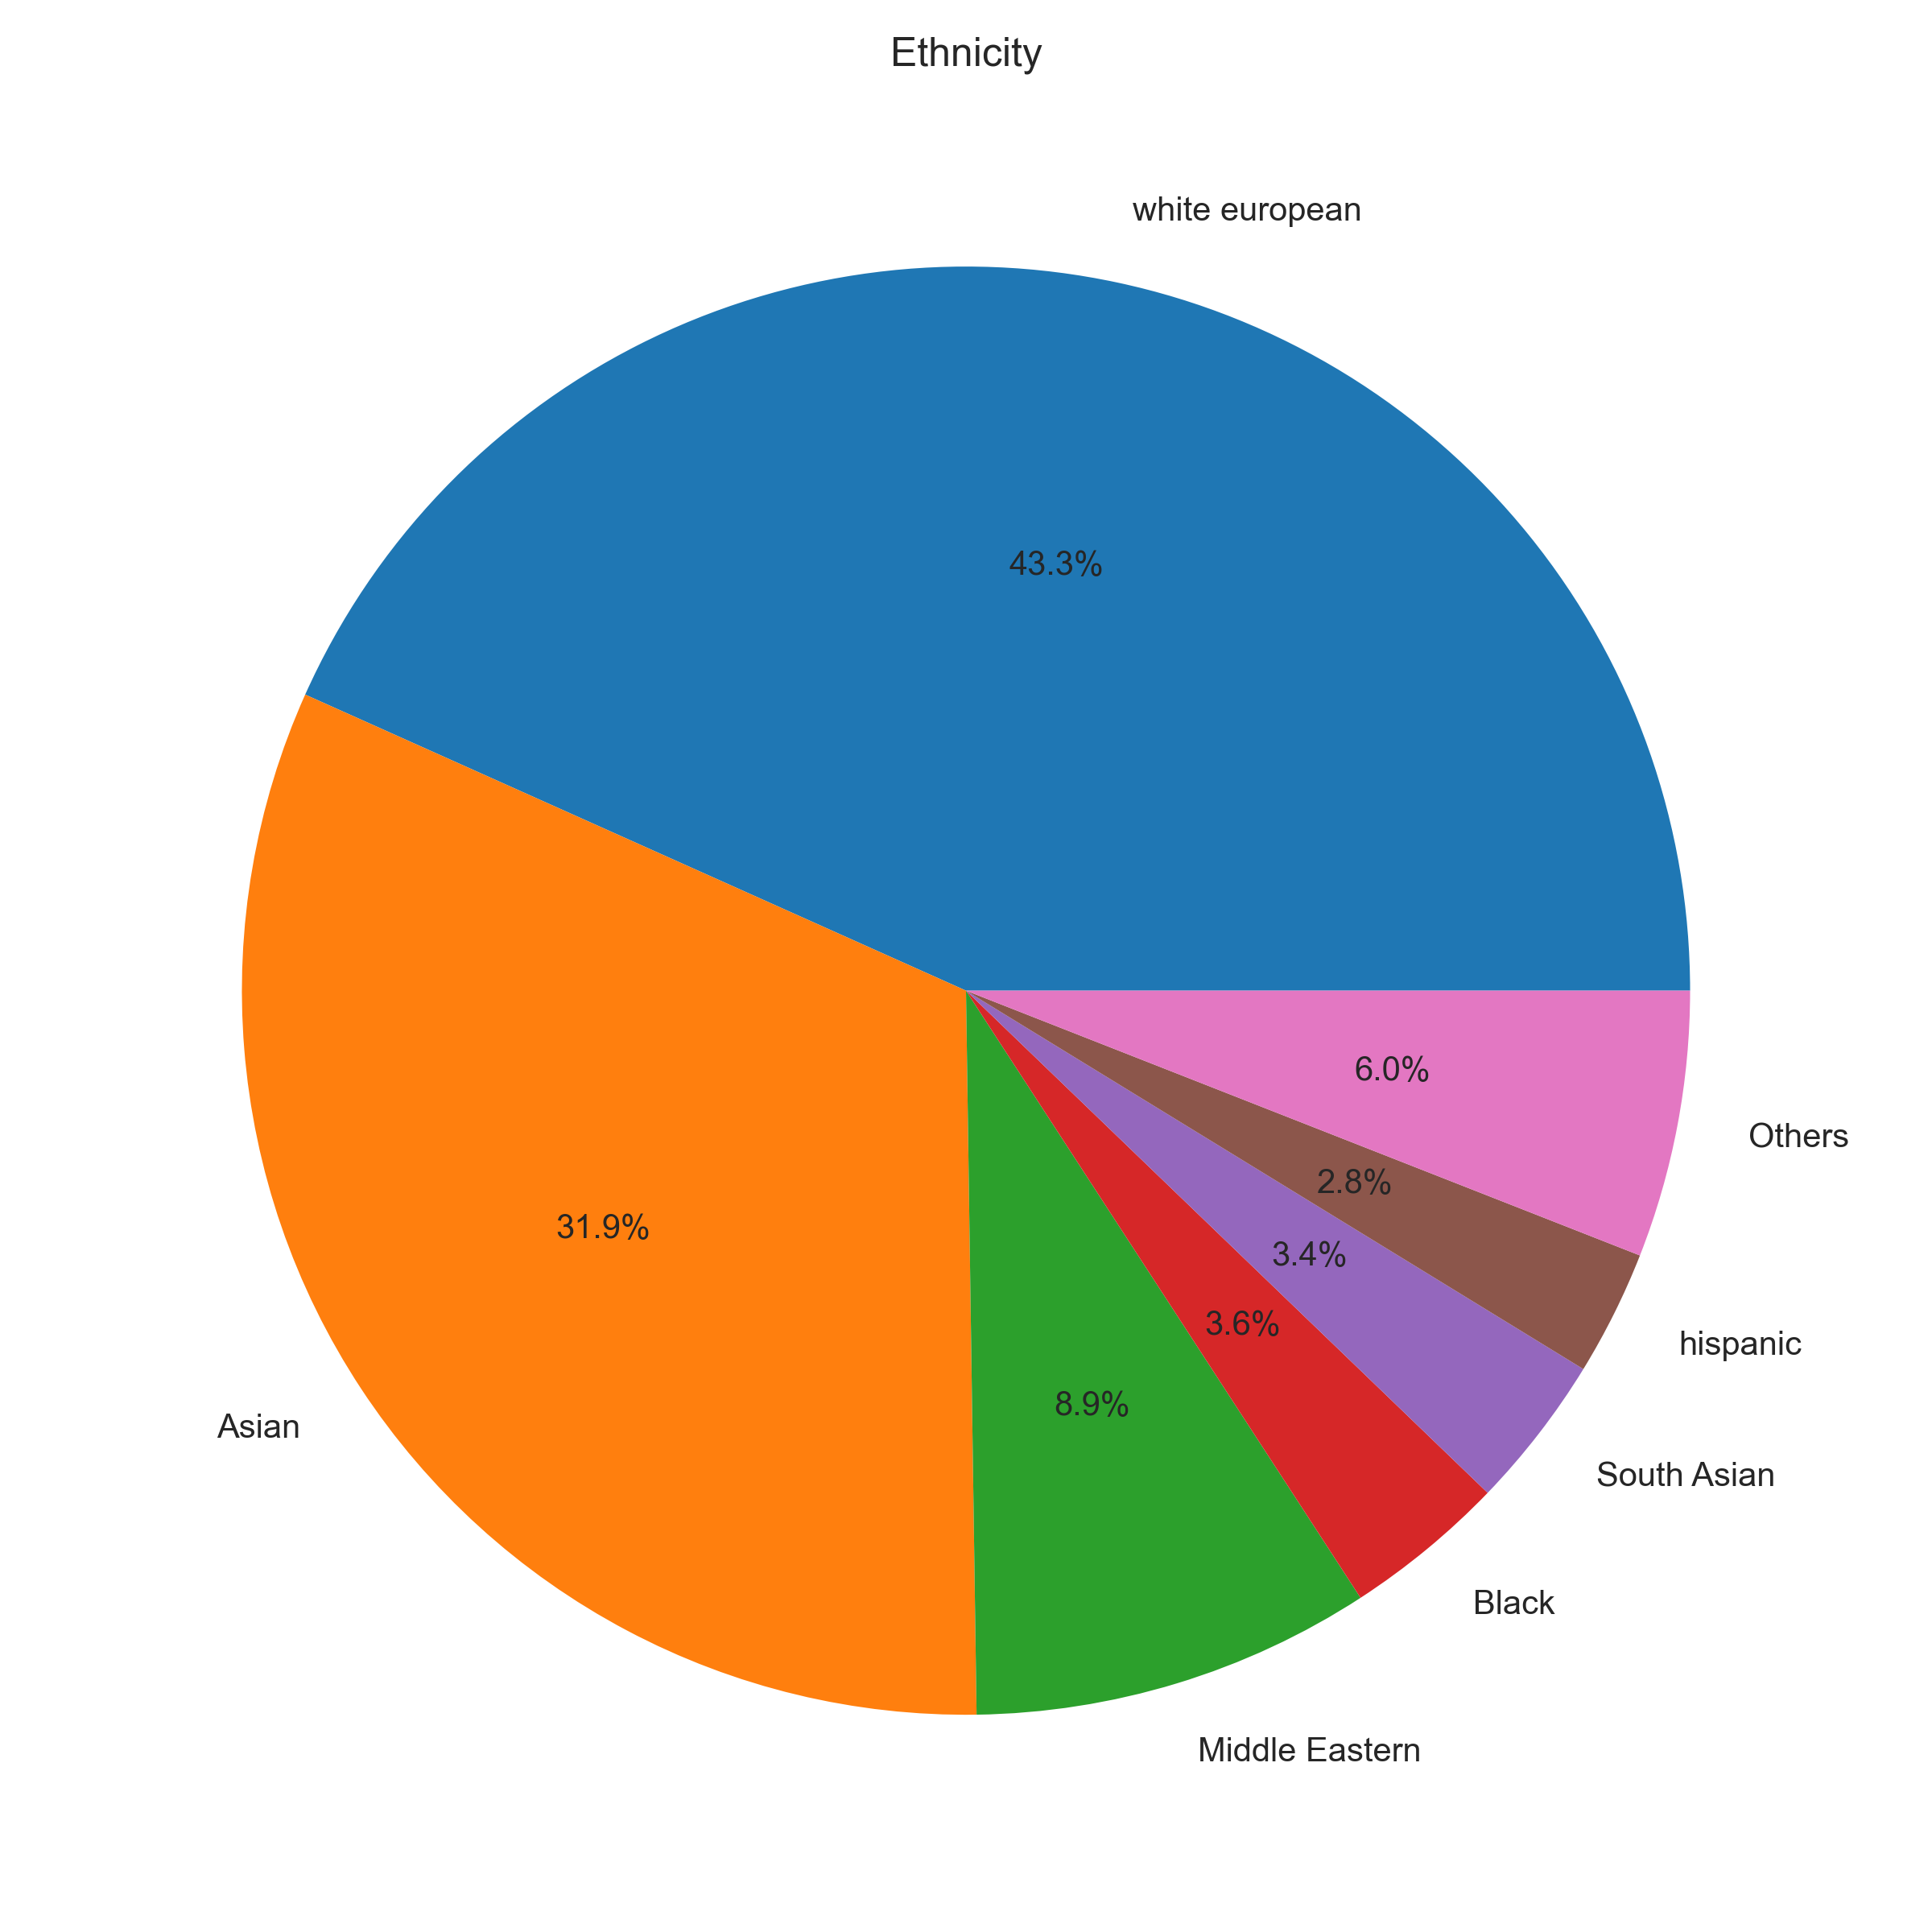
\includegraphics[width=\textwidth]{images/Ethnicity Pie(asd).png}}
                \caption{Participants with ASD from different ethnicity}
                \vspace{1em}
                \label{fig:ethnicity-pie}
            \end{subfigure}
            \caption{Different factors of the participants with ASD}
        \end{figure}

        \begin{figure}[H]
            \centering
            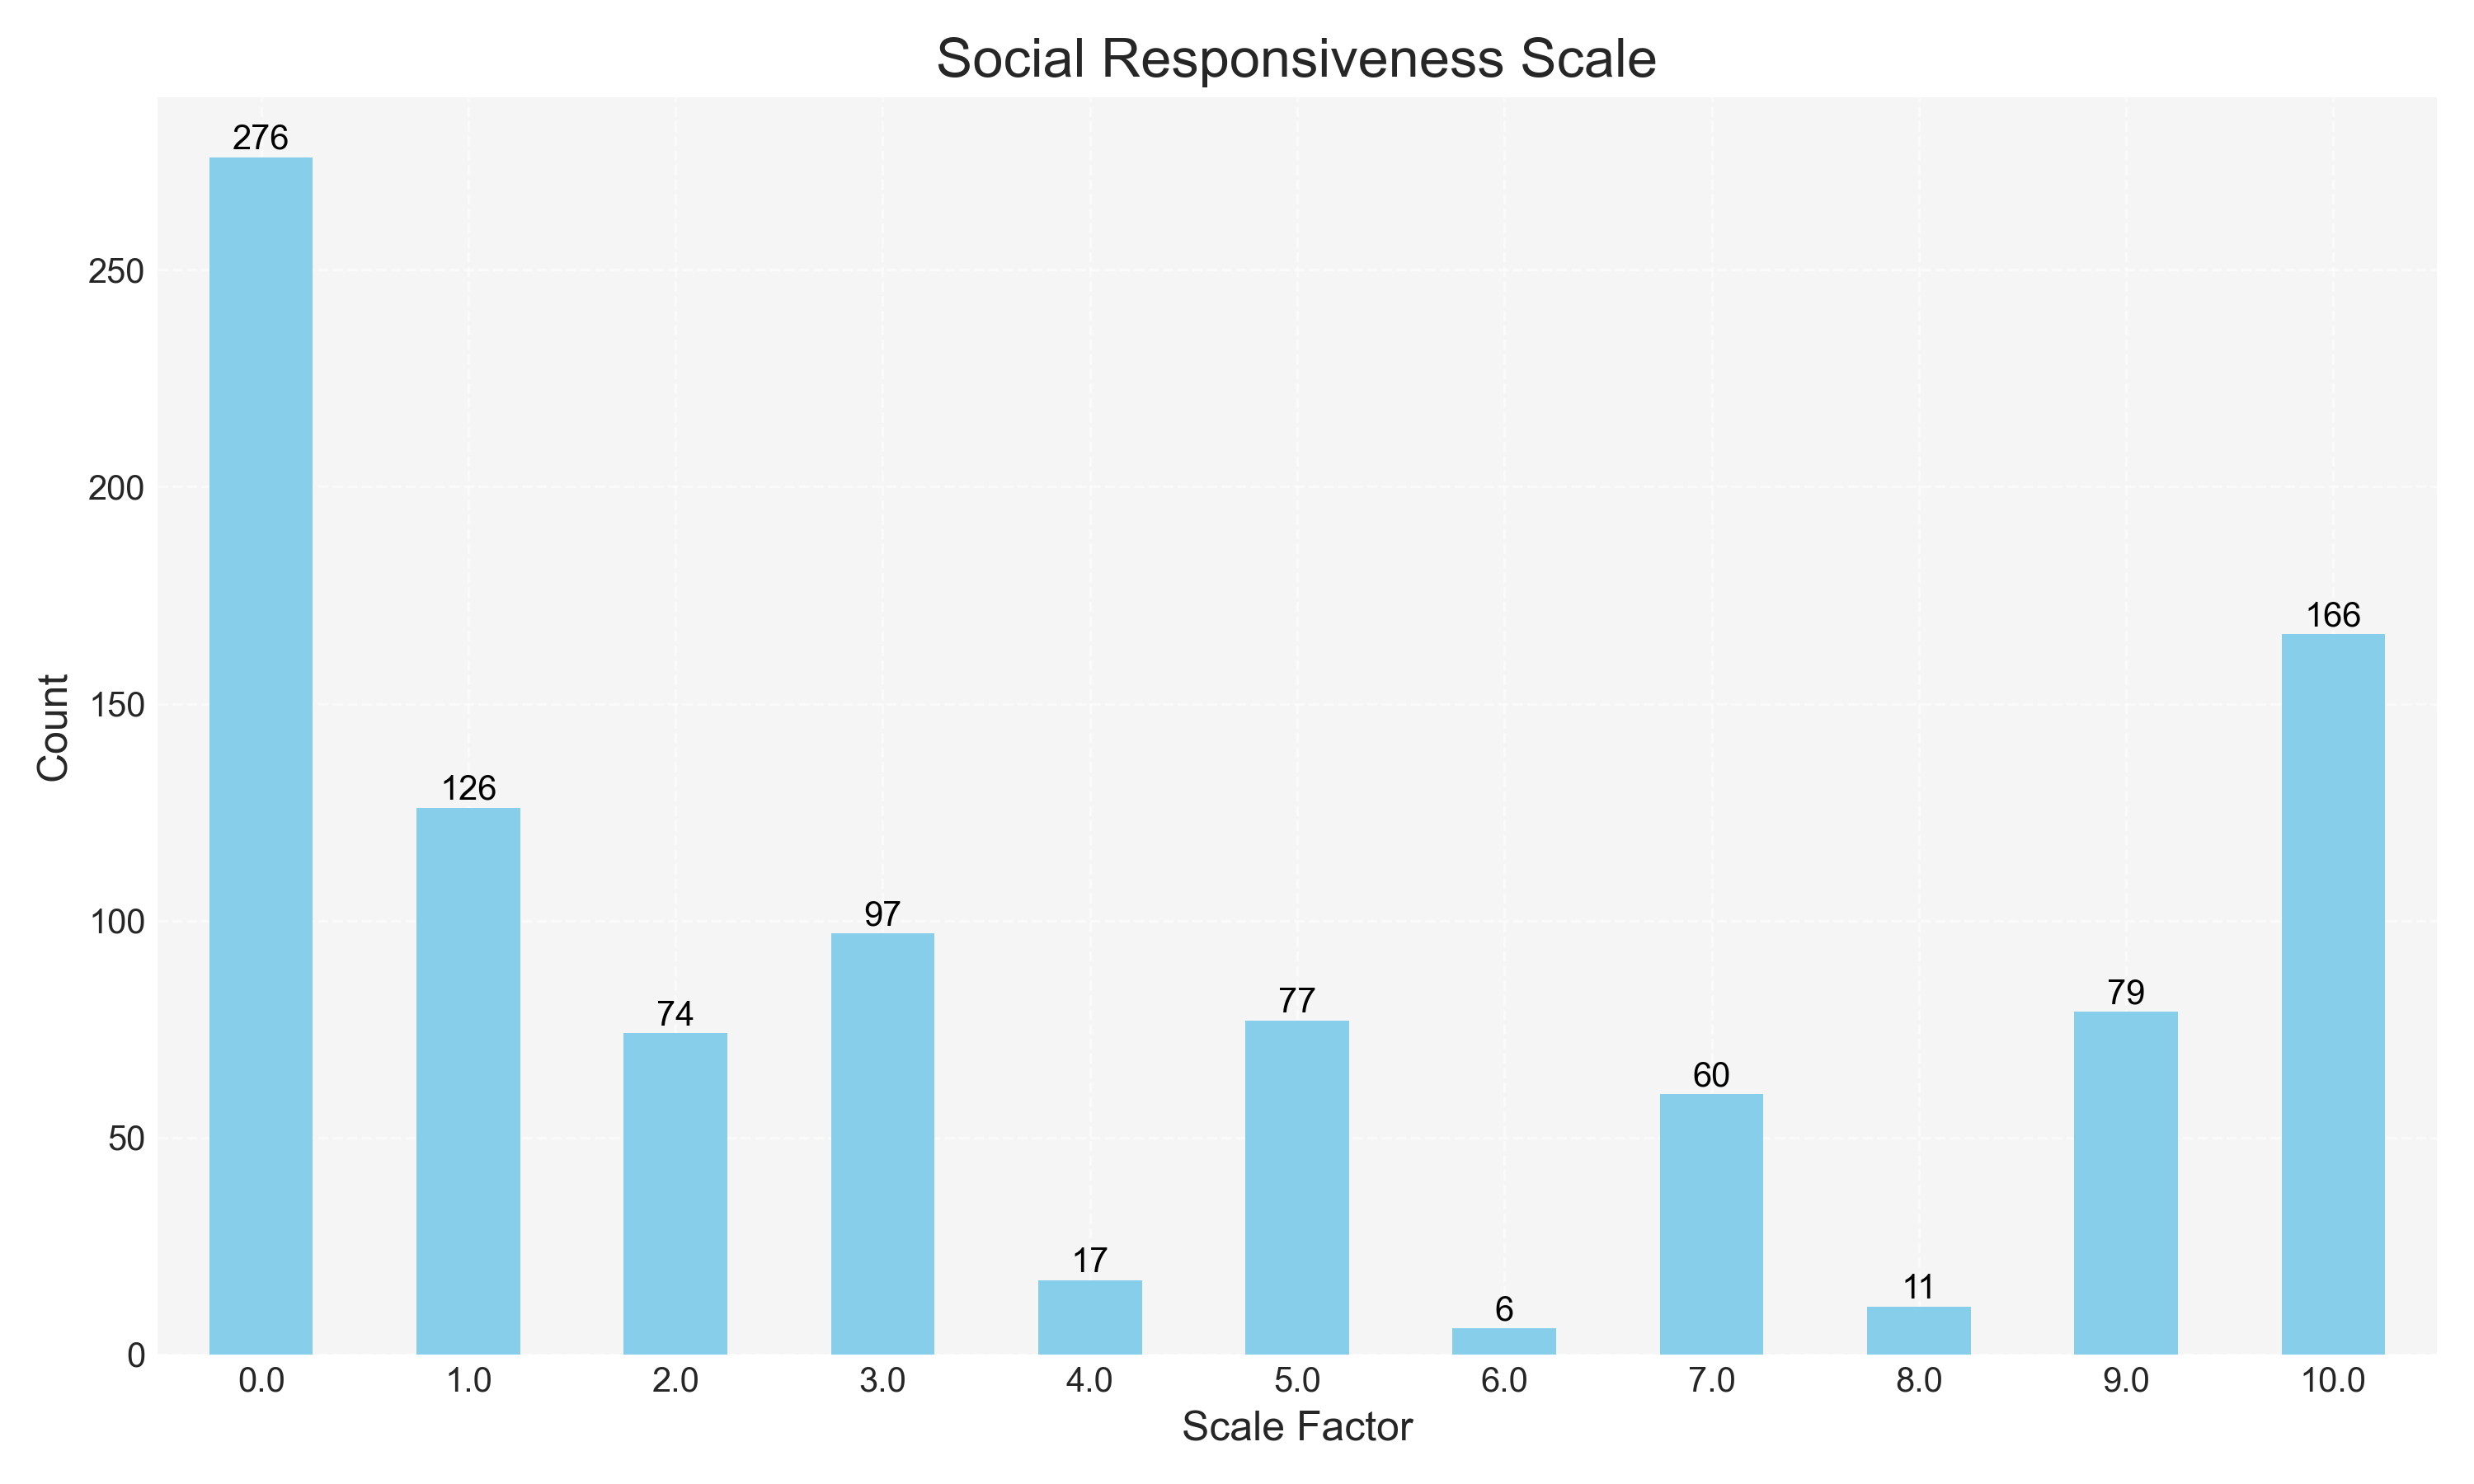
\includegraphics[width=\textwidth]{images/Social Responsiveness Scale(asd).png}
            \caption{Participants' social responsiveness scale (age = more than 3 years old)}
            \label{fig:social-response}
        \end{figure}

\begin{multicols}{2}
\subsection{Algorithms Application}
\hspace*{\parindent}After preprocessing the data and performing data cleaning, as stated, 1937 records made it to the final dataset.The dataset was split into training (80\%) and testing (20\%) purposes. A lot of machine learning algorithms like Logistic Regression, Gradient Boosting, K-nearest Neighbor, Random Forest Classifier, Decision Tree Classifier(entropy and gini), Naïve Bayes(Gaussian), ZeroR Classifier techniques were applied.\\
\hspace*{\parindent}Logistic Regression uses the Linear Regression concept to solve classification problems. To solve the classification problem, it employs the sigmoid function(also known as the logistic function) on linear regression. K-Nearest Neighbor is an instance-based learning technique in which the prediction of a query record is based on the votes provided by the closest k training records. Decision Tree algorithm recursively splits data based on features, creating a tree structure for decisions. Random Forest uses an ensemble of Decision Trees to make predictions. Naïve Bayes algorithm uses a probabilistic approach to make the best prediction.\\
\hspace*{\parindent}Gaussian Naive Bayes classifiers utilize Bayes’ Theorem and Gaussian normal distribution to deduce the output. Naive Bayes also follows essential steps, like generating likelihood coefficients by obtaining the respective probabilities and calculating posterior probability using Naive Bayesian equation as: 
\begin{equation}
     P(A|B) = \frac{P(B|A)\times P(A)}{P(B)}
     \label{naivebayes}
\end{equation}
where, A and B denote discrete events, $P(A|B)$ is the probability of A
given B is true and $P(B|A)$ signifies the probability of event B given A
is true. P(A) and P(B) illustrate the independent probabilities of A and
B, respectively. Finally, the output class is selected with the highest
posterior probability. \\
\hspace*{\parindent}ZeroR is a useful classifier that helps to determine the baseline performance as a benchmark for other classification
methods predicting the majority class.

\subsection{Hyperparameters Optimization}
\hspace*{\parindent}In this work, two hyperparameter optimization techniques (randomized search CV, grid search CV) were used to find the best values for the hyperparameters for the proposed machine learning model. RandomizedSearchCV selects the optimal values by randomizing the search operation. In GridSearchCV, all of the hyperparameters are searched.















\section{Result Analysis}
\hspace*{\parindent}This section discusses the results of the proposed study – detecting the learning rate in children with ASD traits. Accuracy, precision, recall and F1 score are used to measure the performance of various machine learning. Equations \ref{precision} to \ref{accuracy}  were used to determine the performance metrics:
\begin{equation}
    Precision = \frac{TP}{TP+FP}
    \label{precision}
\end{equation}
\begin{equation}
    Recall = \frac{TP}{TP+FN}
    \label{recall}
\end{equation}
\begin{equation}
    F1\,score = 2 \times \frac{precision \times recall}{precision + recall}
    \label{f1}
\end{equation}
\begin{equation}
   accuracy = \frac{TP+TN}{TP+FP+TN+FN}
    \label{accuracy}
\end{equation}\\
where TP,TN,FP,FN are true positives, true negatives, false
positives and false negatives respectively.


% TABLE STARTS
\end{multicols}
\begin{table*}[ht]
  \centering
  \caption{Performance metrics for different algorithms}
  \label{perfmetrics} 
  \vspace{\baselineskip}
  \begin{tabular}{lrrrrr}
  \toprule
  Algorithms & Accuracy & Precision & Recall & F1 score\\
  \midrule
  K-Nearest Neighbour Algorithm(n=5) & $98.38\%$ & $100\%$ & $98.00\%$ & $99.00\%$ \\\\ \hline \addlinespace
  K-Nearest Neighbour Algorithm(n=15) & $97.67\%$ & $100\%$ & $97.00\%$ & $98.00\%$ \\\\ \hline \addlinespace
  Decision Tree Classifier(gini) & $99.48\%$ & $98.00\%$ & $99.00\%$ & $98.00\%$ \\\\ \hline \addlinespace
  Decision Tree Classifier(entropy) & $99.48\%$ & $98.00\%$ & $99.00\%$ & $99.00\%$ \\\\ \hline \addlinespace
  Random Forest Classifier & $99.48\%$ & $100\%$ & $99.00\%$ & $99.00\%$ \\\\ \hline \addlinespace
  Naive Bayes(Gaussian) & $99.03\%$ & $100\%$ & $99.00\%$ & $100\%$ \\\\ \hline \addlinespace
  ZeroR & $55.19\%$ & $54\%$ & $100\%$ & $70\%$ \\\\ \hline \addlinespace
  Linear Regression & $96.48\%$ & $-$ & $-$ & $-$ \\\\ \hline \addlinespace
  Logistic Regression & $99.03\%$ & $-$ & $-$ & $-$ \\\\ \hline \addlinespace
  \end{tabular}\\ 
\end{table*}
\begin{multicols}{2}
% TABLE ENDS

\subsection{Performance Metrics for Different Algorithms}
% description of table
\hspace*{\parindent}Table \ref{perfmetrics} presents a comprehensive evaluation of various machine learning algorithms employed in the development of our model using the data-set. The performance metrics of these algorithms, including Accuracy, Precision, Recall, and F1 Score, are examined, providing critical insights into the diagnostic capabilities of the models.\\
\hspace*{\parindent} Accuracy, as a primary performance indicator, reflects the overall effectiveness of each algorithm in making correct predictions. Remarkably, the algorithms exhibit a wide range of accuracies, with the baseline ZeroR algorithm achieving 55.19\%, while other advanced models attain accuracy levels exceeding 99\% or close to that. \\
\hspace*{\parindent}Precision, which estimates the algorithms' ability to minimize false positives, offers further insights. Several algorithms, including K-Nearest Neighbour Algorithm (n=5), Random Forest Classifier, and Naive Bayes (Gaussian), exhibit perfect precision scores of 100\%. This implies that these models avoid false positive diagnoses entirely, a crucial attribute in clinical decision-making.\\
\hspace*{\parindent}Recall, often referred to as sensitivity, assesses the models' capacity to capture true positive instances. In this context, the algorithms consistently achieve commendable recall rates, consistently surpassing 97\%.\\
\hspace*{\parindent}The F1 Score, a harmonized measure of precision and recall, is utilized to strike a balance between these two key metrics. The algorithms presented robust F1 Scores and notably, Naive Bayes (Gaussian) achieves a perfect F1 Score of 100\% while others remained close to 99\%. \\
\hspace*{\parindent}The Random Forest Classifier emerges as the top-performing algorithm across all metrics, exhibiting near-perfect accuracy while The ZeroR Classifier algorithm performs the least effectively in terms of accuracy and precision. It has the lowest accuracy at 55.19\% and the lowest precision at 54\%. However, it achieves 100\% recall, which means it identifies all actual positive instances, making it highly sensitive but at the expense of specificity. \\
%  description of table 1 ends



% TABLE2 STARTS
\end{multicols}
\begin{table*}[ht]
  \centering
  \caption{Accuracy for different algorithms on dataset after using various hyperparameter optimizers}
  \label{hyperp} 
  \vspace{\baselineskip}
  \begin{tabular}{lrrrrr}
  \toprule
  Algorithms & RandomizedSearch CV(\%) & GridSearch CV(\%)\\
  \midrule
  Random Forest Classifier(gini) & $99.48\%$ & $99.48\%$ \\\\ \hline \addlinespace
  Random Forest Classifier(entropy) & $99.48\%$ & $99.48\%$ \\\\ \hline \addlinespace
  \end{tabular}
\end{table*}
\begin{multicols}{2}
% table 2 ends


\subsection{Performance Metrics for Different Algorithms using Hyperparameter Optimization}
% table 2 description starts
\hspace*{\parindent} Table \ref{hyperp} presents accuracy metrics for different machine learning algorithms after applying two different hyperparameter optimization techniques: Randomized-Search and Grid-Search. These techniques aim to fine-tune the hyperparameters of the algorithms to improve their predictive performance.\\
\hspace*{\parindent}The Algorithm column lists the machine learning algorithms under evaluation. In this case, ``Random Forest Classifier'' is the algorithm used for both gini and entropy criteria. \\
\hspace*{\parindent}The Randomized-Search column represents the accuracy achieved by the Random Forest Classifier when hyperparameter optimization is performed using the Randomized-Search method. Accuracy is a crucial metric, as it indicates the proportion of correctly predicted outcomes. In both cases (gini and entropy criteria), the Randomized-Search achieves a high accuracy of 99.48\%. This suggests that the Randomized-Search method was successful in fine-tuning the hyperparameters of the Random Forest Classifier, resulting in highly accurate predictions.\\
\hspace*{\parindent}The Grid-Search column represents the accuracy achieved by the Random Forest Classifier when hyperparameter optimization is performed using the Grid-Search method. Similar to the Randomized-Search, the Grid-Search also achieves an accuracy of 99.48\% for both gini and entropy criteria. This indicates that the Grid-Search method produces identical accuracy levels to the Randomized-Search.
% table 2 description ends

\subsection{Classifier Accuracy using Different Algorithms in both Train and Test set}

\hspace*{\parindent}In this section in Figure \ref{acc1} and \ref{acc2}, we present an analysis using bar-chart of the accuracy scores achieved by various machine learning algorithms in the context of diagnosing Learning Disorders in children. The accuracy scores are evaluated on both the test and training datasets, shedding light on the effectiveness of these algorithms in this critical domain.\\
% \hspace*{\parindent}
% When evaluating the performance of these classifiers on the test dataset, Logistic Regression emerged as the top performer, achieving the highest test accuracy of 99.48 percent. Random Forest closely followed with an impressive test accuracy of 99.22 percent. K-Nearest Neighbor(k=15) displayed competitive accuracy at 98.71 percent, outperforming (k=5) at 98.19 percent along with Decision Tree (Gini) and Decision Tree (Entropy) of score 98.45 percent. ZeroR, serving as our baseline, achieved the lowest test accuracy of 53.86 percent. \\


\end{multicols}
    \noindent
    \begin{minipage}{\textwidth}
        \begin{figure}[H]
            \centering
            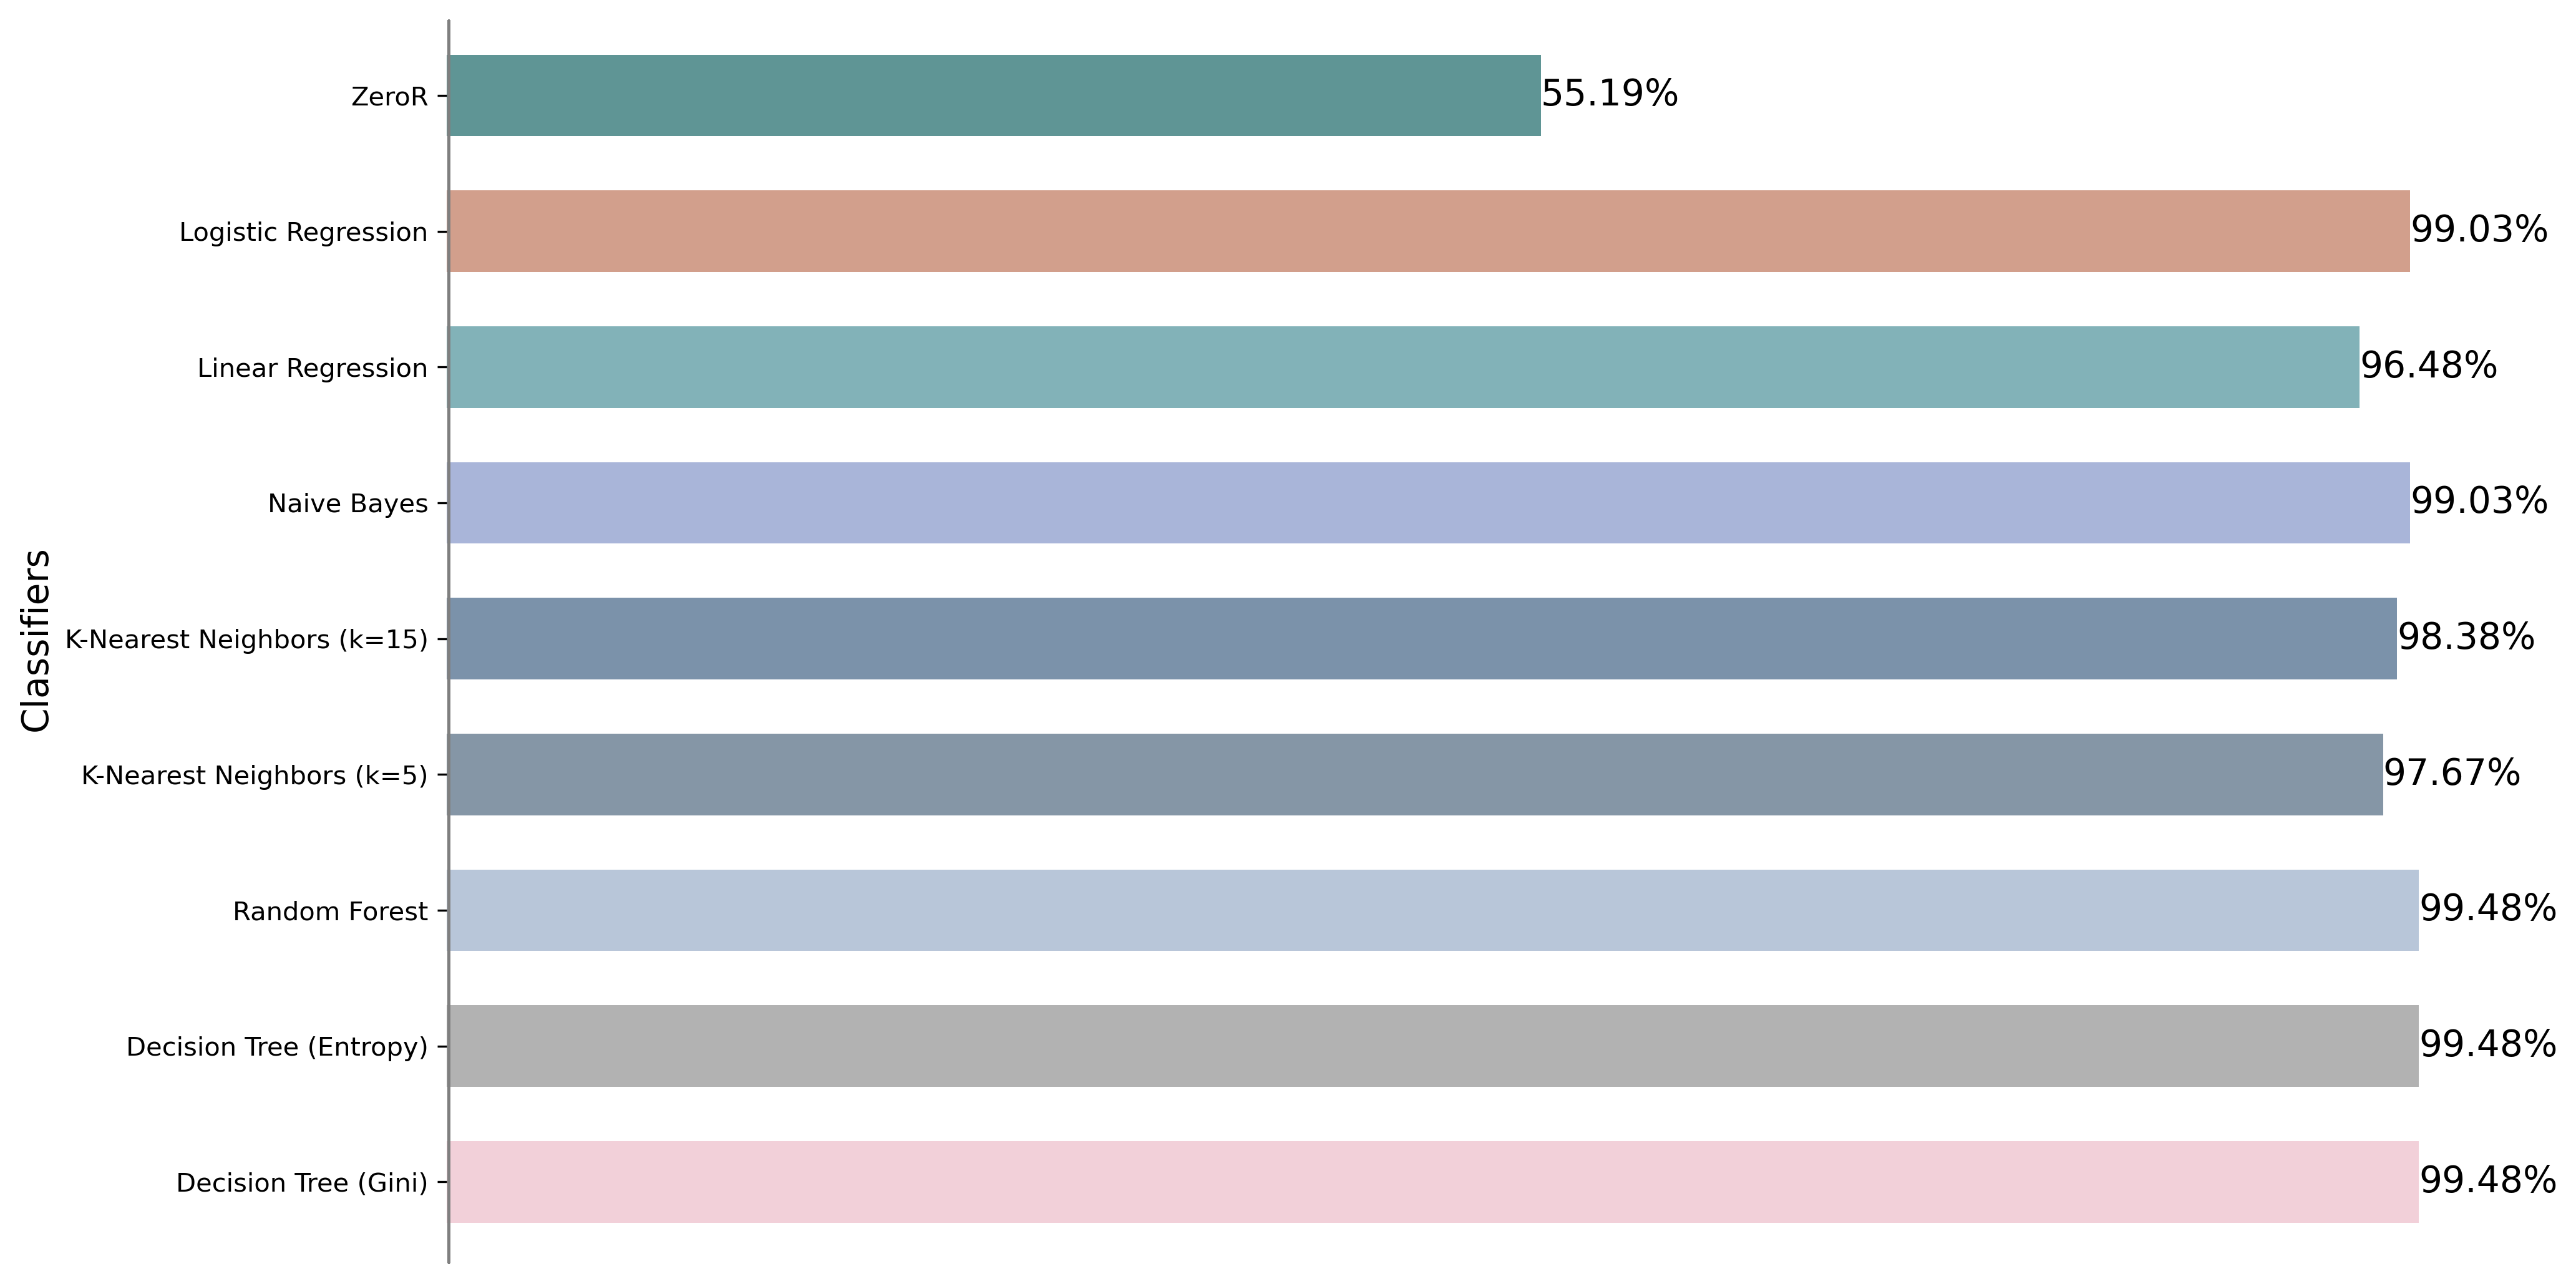
\includegraphics[width=0.9\textwidth]{images/bar_chart.png}
            \caption{Percentage Accuracy of Algorithms represented in a Bar-Chart}
            \vspace{0.1em}
            \label{acc1}
        \end{figure}
        \begin{figure}[H]
            \centering
            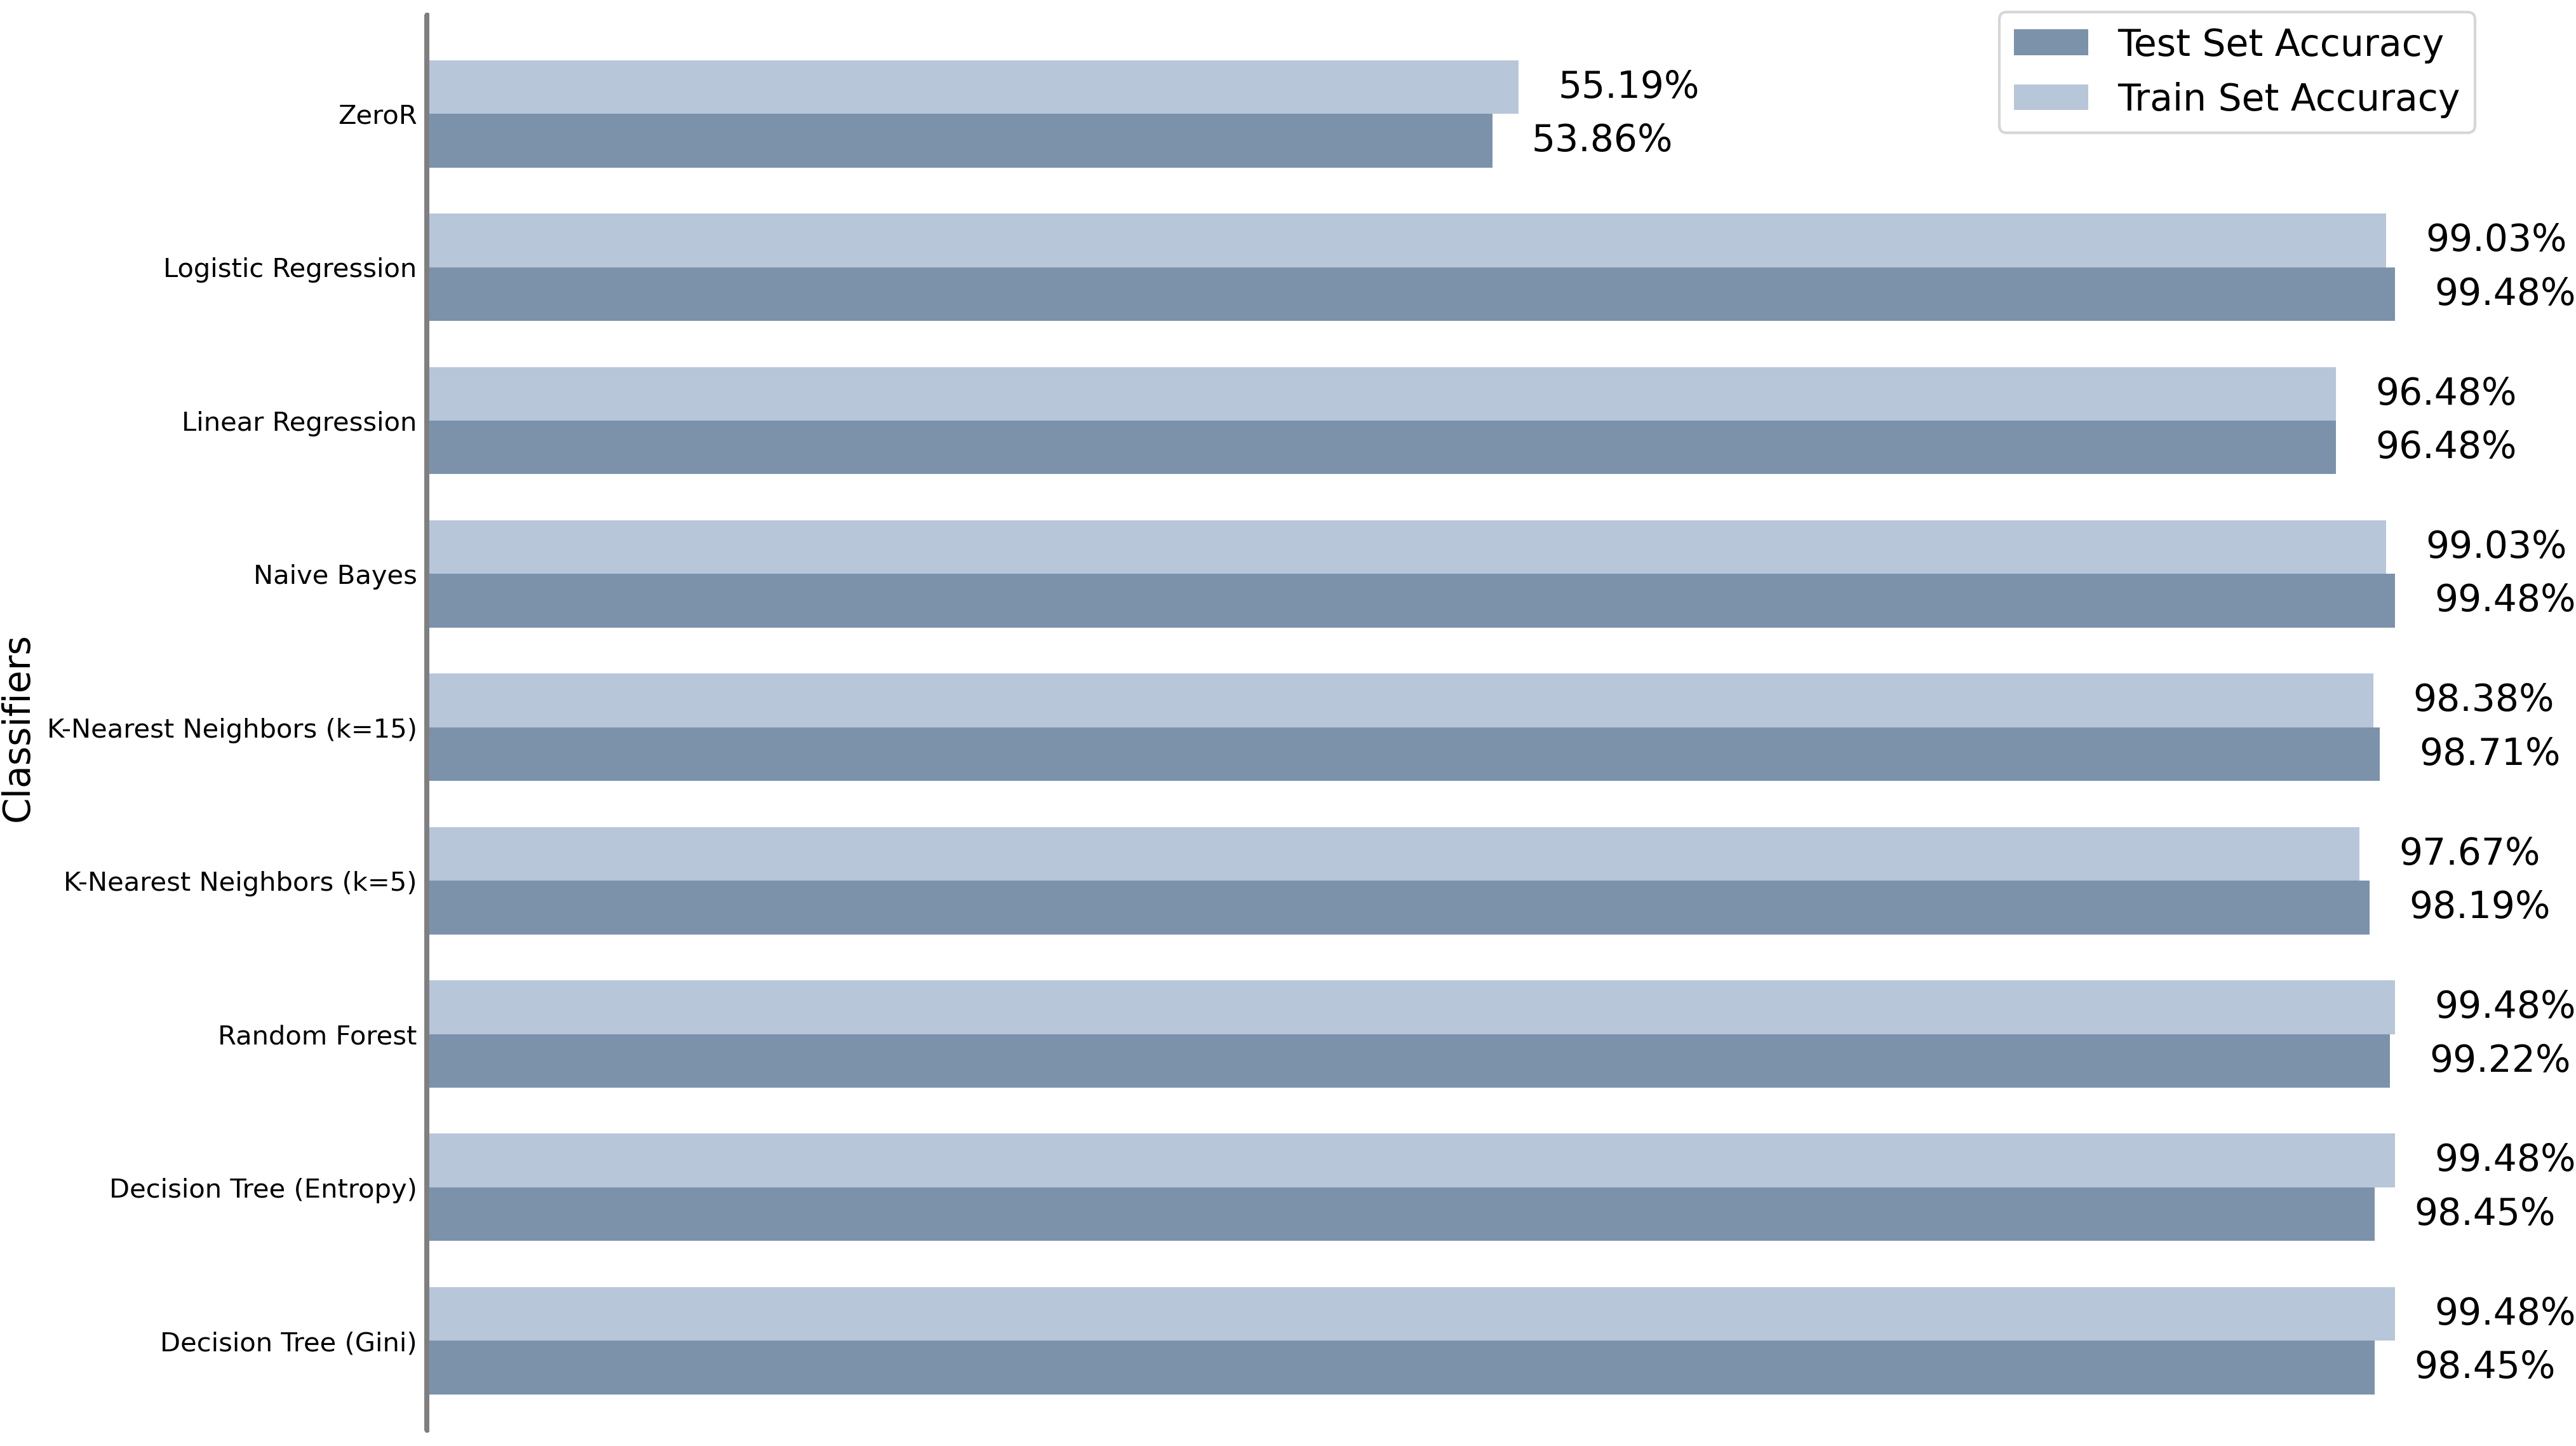
\includegraphics[width=0.9\textwidth]{images/classifier_accuracy_horizontal.png}
            \caption{Percentage Accuracy of Algorithms represented in a Bar-Chart for both Train and Test Set}
            \vspace{0.1em}
           \label{acc2}
        \end{figure}
    \end{minipage}
\begin{multicols}{2}


\subsection{Cross Validation Techniques}

\hspace*{\parindent}Cross-validation is a critical process in machine learning, allowing us to assess the performance and generalization of our models.\\
\hspace*{\parindent}
Firstly we attempted HoldOut Validation which is a straightforward approach where the dataset is split into training and testing sets. It yielded an accuracy of 98.96\%, indicating a commendable model performance. However, the reliance on a single random split can make it less reliable.\\
\hspace*{\parindent}
 Stratified Hold-Out Validation is an improvement over basic HoldOut. It ensures that the class distribution in both the training and testing sets is similar to the original dataset. The accuracy score of 99.22\% suggests that this technique better preserves the class balance and provides slightly better performance.\\
\hspace*{\parindent}
 Kfold Validation involves dividing the dataset into "k" subsets and using each of them as a testing set while the remaining "k-1" subsets are used for training. The process is repeated "k" times, and the results are averaged. The accuracy score of 98.76\% represents the average performance over multiple splits. It provides a more robust estimate of the model's generalization.\\
 \hspace*{\parindent}
 LOOCV is an extreme case of Kfold Validation where "k" is equal to the number of data points. In each iteration, one data point is used for testing, and the remaining points are used for training. This technique provides a thorough assessment of the model's performance. The accuracy score of 98.55\% suggests that the model performed slightly worse, possibly due to the high variance in the evaluation process.\\
 \hspace*{\parindent}
 Figure \ref{cross} shows the differences between the Cross Validation results. Compared to the rest, Stratified Hold-Out Validation emerges as the best performer, preserving class balance and demonstrating high accuracy.\\
 \hspace*{\parindent}\\

\end{multicols}
    \noindent
    \begin{minipage}{\textwidth}
        \begin{figure}[H]
            \centering
            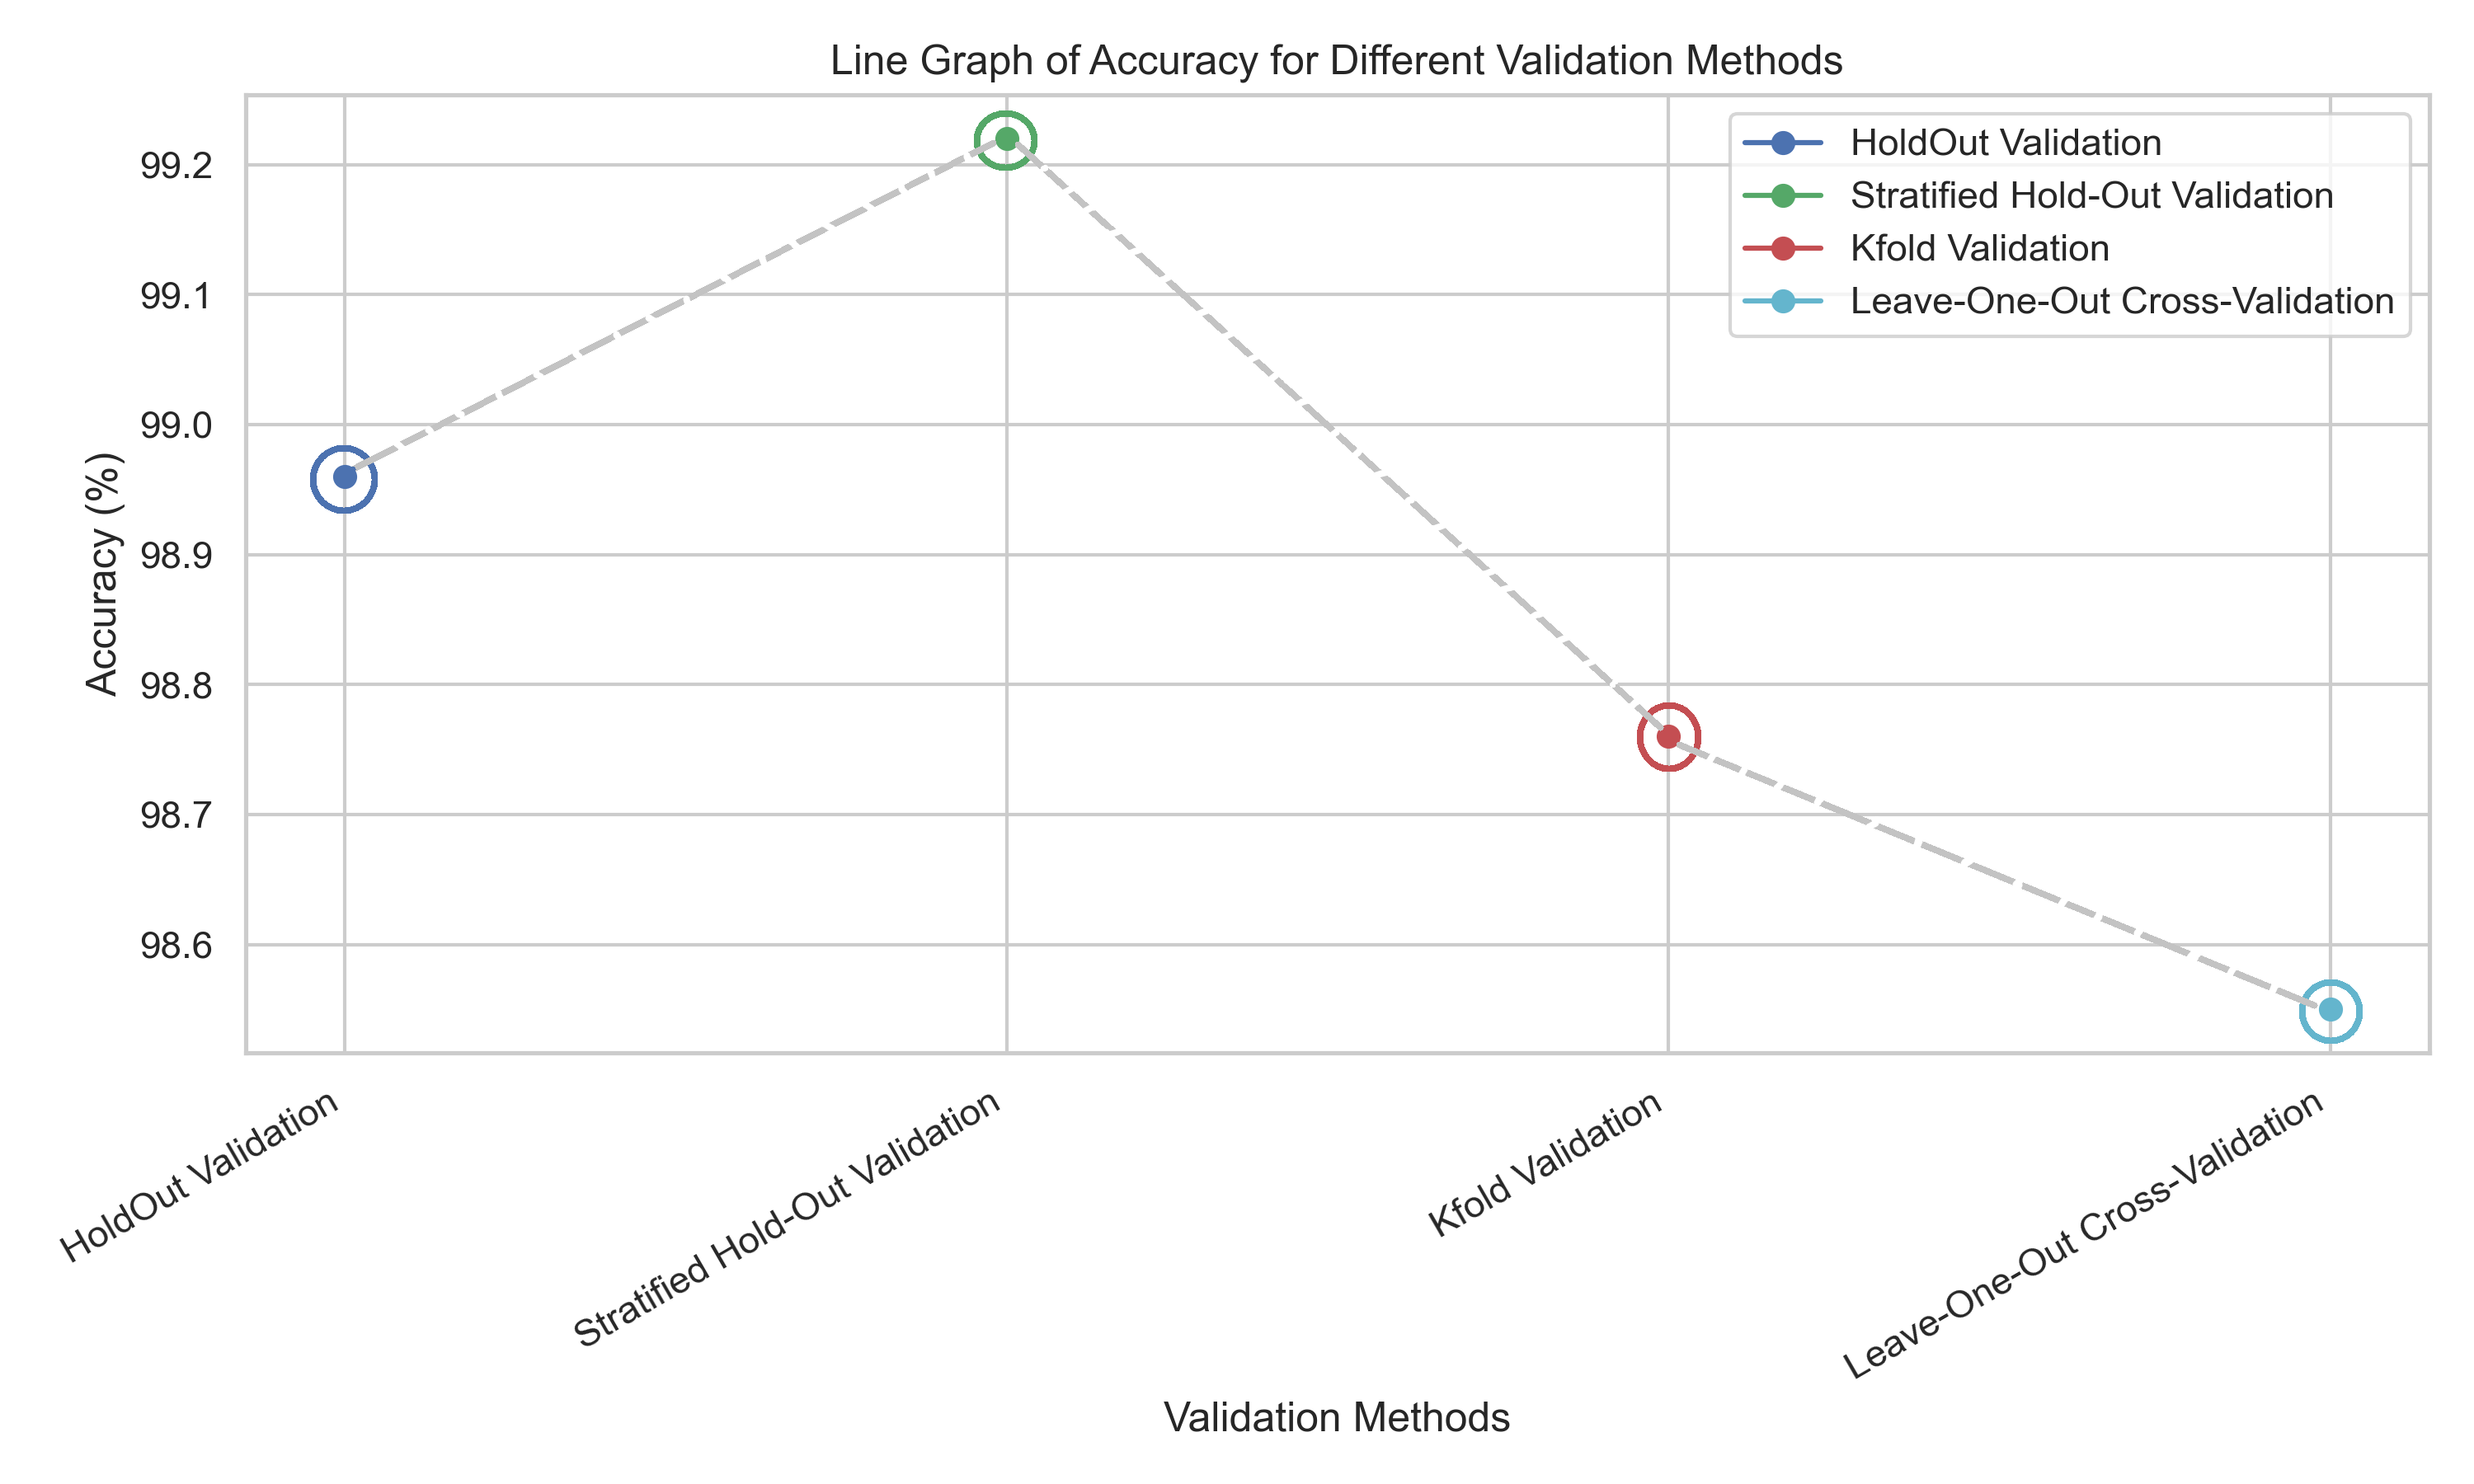
\includegraphics[width=1.\textwidth]{images/colorful_line_graph.png}
            \caption{Difference in Cross Validation Techniques displayed using line graph}
            \vspace{0.1em}
           \label{cross}
        \end{figure}
        
    \end{minipage}
    
\begin{multicols}{2}



\subsection{Explainable AI(XAI) using LIME}

\hspace*{\parindent}In this study, we applied Local Interpretable Model-agnostic Explanations (LIME) as part of our broader framework for Explainable Artificial Intelligence (XAI). As XAI is used for it's set of techniques and methodologies to make the model more transparent, LIME focuses on explaining individual predictions made by machine learning models, regardless of the model's complexity. It is a powerful tool that can be used to improve the diagnosis, treatment, and understanding of learning disorders in children. By using LIME we aimed to identify the features that are most important to learning disorder. These local models provide explanations for why a particular prediction was made.\\
\hspace*{\parindent}
Figure \ref{limeai} provides a concise overview of the LIME results, highlighting the features that influence the prediction probabilities and their respective scores. It helps to understand the key factors contributing to the model's predictions regarding Learning Disorder. We used Random Forest since it gave the best results. \\


\end{multicols}
    \noindent
    \begin{minipage}{\textwidth}
        \begin{figure}[H]
            \centering
            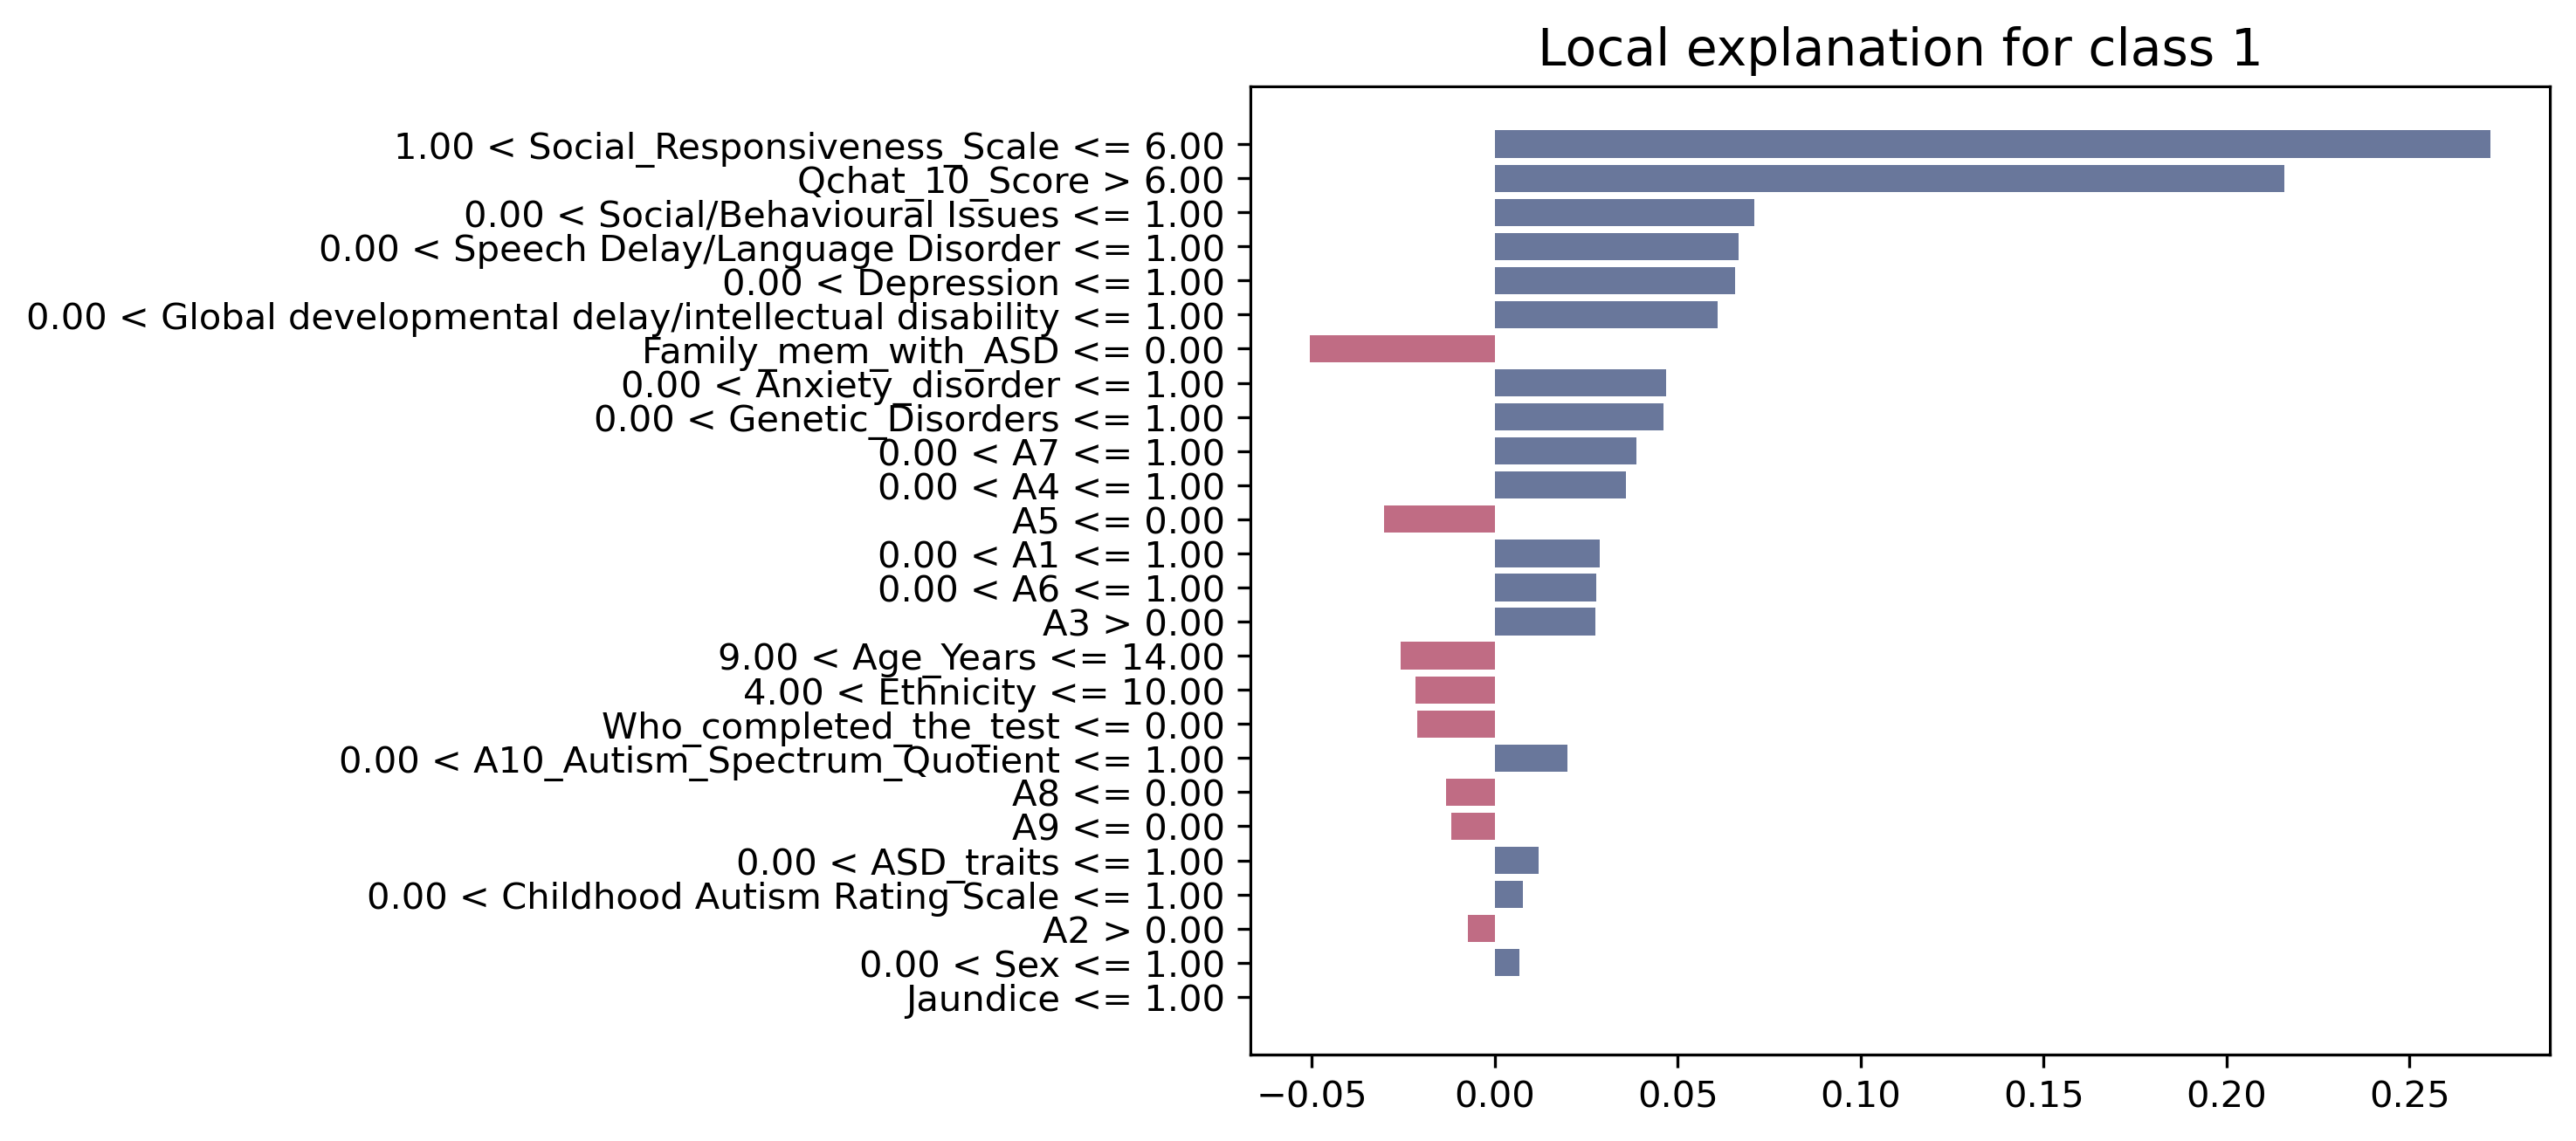
\includegraphics[width=1\textwidth]{images/lime_explanation_hd.png}
            \caption{Prediction Probability Interpretation using LIME Explainable AI}
            \vspace{0.1em}
            \label{limeai}
        \end{figure}
    \end{minipage}
\vspace{1\baselineskip}
\begin{multicols}{2}

\section{Discussion}
\hspace*{\parindent} This study aimed to develop a robust machine learning model to accurately predict learning disorders in children. At first we determined what to predict from our dataset, then after much deliberation decided to focus on predicting the likelihood of learning disorders in children with ASD traits. Most people are unaware that up to 80\% of autistic individual also have learning disabilities. Hence our motive was driven by the critical importance of identifying learning disorders early to mitigate the potentially adverse effects on a child's development as well as to to provide effective treatment and support. \\
\hspace*{\parindent} We used a dataset of 1985 children with ASD traits, and we evaluated a variety of machine learning algorithms. Our findings revealed outstanding accuracy in predicting learning disorders among children with ASD traits. Algorithms we used including K-Nearest Neighbors, Decision Tree Classifiers (using both Gini and Entropy criteria), Random Forest, and Naive Bayes (Gaussian) achieved accuracy levels surpassing 99\%. This high level of accuracy emphasizes the ability of these algorithms in accurately identifying individuals at risk of developing learning disorders.\\
\hspace*{\parindent} In addition to the prominent accuracy achieved in our study, the integration of cross-validation techniques significantly enhanced the robustness and reliability of our machine learning model. Cross-validation methods, such as Stratified Hold-Out, Kfold, and Leave-One-Out Cross-Validation, were instrumental in ensuring the model's generalization capabilities. These techniques not only assessed the model's performance but also provided valuable insights into its consistency across various data splits. By leveraging cross-validation, we minimized the risk of overfitting and gained a deeper understanding of the model's ability to detect learning disorders in children with ASD traits.\\
\hspace*{\parindent} In addition to training the model with different techniques and checking its performance, we also explored explainable AI (XAI) using the Local Interpretable Model-agnostic Explanations (LIME) framework. This helped us not only understand how well various algorithms could make predictions but also made it clear why the model made specific decisions. It provided a transparent window into the model's thought process and made our findings more reliable and understandable.\\
\hspace*{\parindent} Our research offers valuable insights into the detection and prediction of learning disorders in children with ASD traits. By combining rigorous methodologies and the power of machine learning, we have demonstrated the potential to identify those at risk of learning disorders with high accuracy.\\




\section{Limitations of the work}
\hspace*{\parindent}This article presents a novel approach of predicting learning disorder in children with ASD traits using machine learning models and was applied to children aged 1 to 18 years old, from various parts of the world. However, the work has experienced a number of challenges:
\begin{itemize}
    \item The dataset size might be a constraint. With 1937 values, it could be challenging to capture the full diversity of ASD traits in children. A larger and more diverse dataset could enhance the generalizability of our findings.
    \item The age range of 1 to 18 years of our participants is quite broad. Children undergo significant developmental changes during this period, and the factors influencing learning disorders may vary. It might be beneficial to consider subgroups within this range to provide more nuanced insights.
    \item The reliance on a Kaggle dataset could introduce biases, as the data might not be fully representative of the broader population. 
    \item The application of machine learning models to predict learning disorders raises ethical concerns. The potential for misdiagnosis or stigmatization should be addressed, and the model's real-world implications on children's lives should be carefully considered.
\end{itemize}

\section{Conclusion and Future Scope}
\hspace*{\parindent}This study presents various machine learning methods for assessing the predictability of learning disorder among children exhibiting Autism Spectrum Disorder (ASD) traits. In addition, the study explores various other reasons that help us in determining the occurrence of learning disorder among these children. Through the utilization of a carefully curated dataset and the application of various machine learning algorithms, we achieved remarkable accuracies, notably 99.48\% with both decision tree and random tree classifiers, which were noted as the better models for evaluating learning disorder. The incorporation of hyperparameter optimization and the interpretability framework LIME further enhances the robustness and explainability of our predictive models.\\
\hspace*{\parindent}As we look to the future, avenues for improvement and expansion become apparent. First and foremost, obtaining a more extensive and diverse dataset, representative of various demographics, would significantly strengthen the external validity of our models. Exploring the integration of longitudinal data could offer valuable insights into the developmental trajectories of ASD traits and their correlation with learning disorders over time. We aim to collect dataset from children with ASD traits from Bangladesh, so that we can get a better prediction in the future.\\
\hspace*{\parindent}In essence, while this research marks a significant stride in the direction of early detection of learning disorders in children with ASD traits, it is a step in an ongoing journey. Through continuous refinement, and collaborative efforts, the pursuit of improving the academic and social outcomes for these children remains a dynamic and promising avenue for future research.





\end{multicols}

\vspace{3\baselineskip}

\bibliographystyle{unsrt}
\bibliography{reference}
\end{document}
